\documentclass{beamer}
%
% Choose how your presentation looks.
%
% For more themes, color themes and font themes, see:
% http://deic.uab.es/~iblanes/beamer_gallery/index_by_theme.html
%

\mode<presentation>
{
  \usetheme{Darmstadt}      % or try Darmstadt, Madrid, Warsaw, ...
  \usecolortheme{beaver} % or try albatross, beaver, crane, ...
  \usefonttheme{default}  % or try serif, structurebold, ...
  \setbeamertemplate{navigation symbols}{}
  \setbeamertemplate{caption}[numbered]
} 

\usepackage[backend=bibtex]{biblatex}
\addbibresource{bibliography.bib}
\newtheorem*{remark}{Remark}
\usepackage[english]{babel}
\usepackage[utf8x]{inputenc}
\usebackgroundtemplate{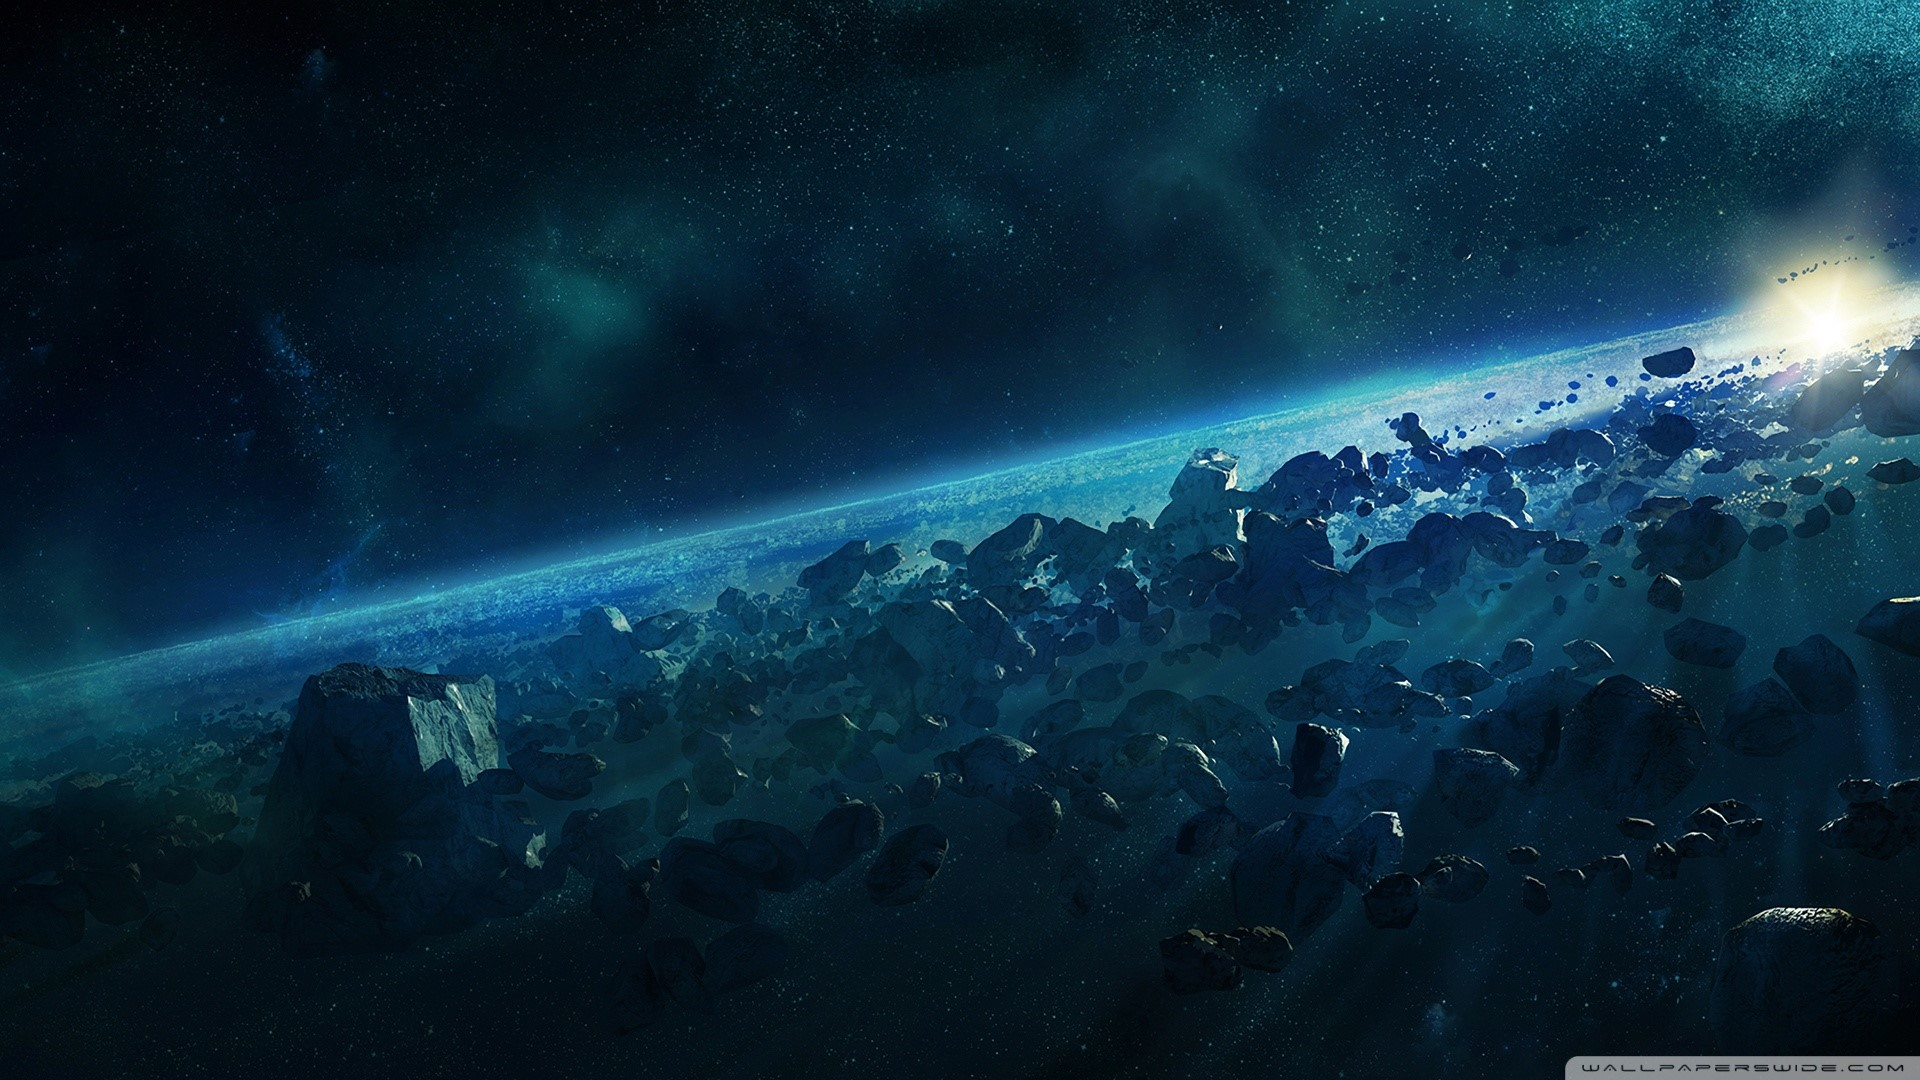
\includegraphics[width=\paperwidth]{Pic/Intro.jpg}}
\title[Hazardous asteroids forecast via Markov random fields]{Hazardous asteroids forecast via Markov random fields}
\subtitle{Project for the exam: Probabilistic Modelling (DSE)}
\author{Marzio De Corato}
\date{\today}

\begin{document}

\begin{frame}
\vspace{+4 cm}  \titlepage
\end{frame}

\usebackgroundtemplate{ } 

% Uncomment these lines for an automatically generated outline.
%\begin{frame}{Outline}
%  \tableofcontents
%\end{frame}

\section{Intro}

\begin{frame}{Introduction}

\begin{itemize}
\item \textbf{Final Goal} Assessment of forecasts and interpretability for different machine learning algorithms, including the probabilistic models
\item \textbf{Method} Use a dataset for which the laws that interconnect the different features are known from general principles
\item \textbf{Dataset} CNEOS asteroids dataset for more than 3500 asteroids
\item \textbf{Theoretical laws} Celestial mechanics
\item \textbf{Algorithms involved - probabilistic models} GLASSO, mgm, minforest, mmod
\item \textbf{Algorithms involved - others} Random forest, Support Vector Machines, Quadratic Discriminant Analysis, Logistic Regression  

\end{itemize} 

\end{frame}

\section{Celestial mechanics}


\begin{frame}{Celestial mechanics \cite{murray1999solar}: equations of motion}

\begin{center}
Lets Consider the interaction between a planet of mass $m_{1}$ at the  position $r_{1}$ (inertial frame) and an asteroid of mass $m_{2}$  at the position $r_{2}$
\end{center}


\begin{equation}
\textbf{F}_{1}=\mathcal{G} \cdot \frac{m_{1}m_{2}}{r^{3}}\textbf{r}=m_{1} \ddot{\textbf{r}}_{1}\quad \textbf{F}_{2}=-\mathcal{G} \cdot \frac{m_{1}m_{2}}{r^{3}}\textbf{r}=m_{1} \ddot{\textbf{r}}_{2}
\end{equation}

 
If we consider the motion of the second item with respect to the first one 
 
\begin{equation}
\ddot{\textbf{r}}=\ddot{\textbf{r}}_{2}-\ddot{\textbf{r}}_{1} \quad \mu=\mathcal{G}(m_{1}+m_{2})
\end{equation}

\begin{equation}
\dfrac{d^{2}\textbf{r}}{dt^{2}}+\mu\dfrac{\textbf{r}}{r^{3}}=0
\end{equation}

\begin{center}
$\textbf{r} \times \ddot{ \textbf{r}}=0  \implies $ $\textbf{r}$  and $\dot{\textbf{r}}$ lies in the same plane

\end{center}
\end{frame}

\begin{frame}{Celestial mechanics \cite{murray1999solar}: equations of motion}
\begin{center}
With polar coordinates  $\hat{\textbf{r}}$ and $\hat{\boldsymbol{\theta}}$
\end{center}
\begin{equation}
\textbf{r}=r\hat{\textbf{r}}
\end{equation}

\begin{equation}
\dot{\textbf{r}}=\dot{r}\hat{\textbf{r}}+r\dot{\theta}\hat{\boldsymbol{\theta}}
\label{eq_dyn_nop}
\end{equation}

\begin{equation}
\ddot{\textbf{r}}=\left(\ddot{r}-r\dot{\theta}^{2}\right)\hat{\textbf{r}}+\left[\dfrac{1}{r}\frac{d}{dt}\left(r^{2}\dot{\theta}\right)\right]\hat{\boldsymbol{\theta}}
\end{equation}

\begin{equation}
\textbf{h}=r^{2}\dot{\theta}\hat{\textbf{z}}
\end{equation}


\begin{equation}
h=r^{2}\dot{\theta}
\end{equation}

\end{frame}


\begin{frame}{Celestial mechanics \cite{murray1999solar}: $2^{th}$ Kepler law}

\begin{figure}[h]
\begin{center}
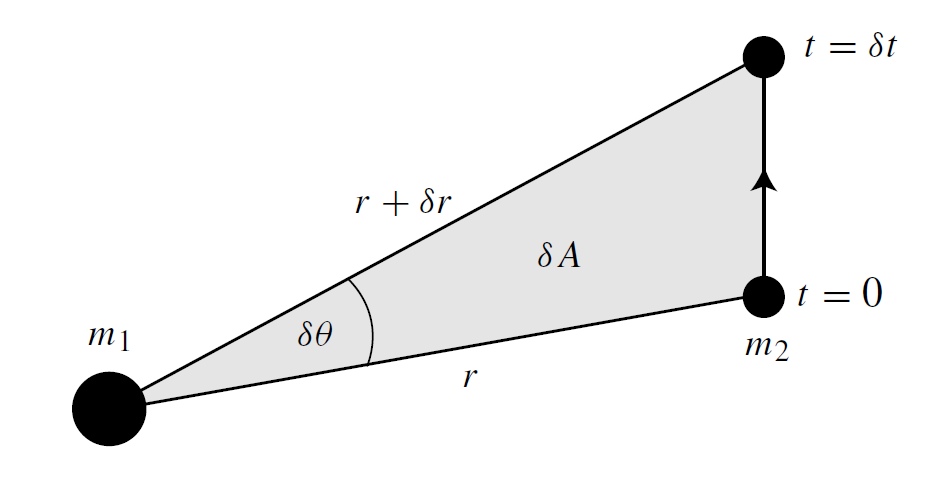
\includegraphics[width=0.3\textwidth]{Pic/Area_dynamics.png}
\caption{\cite{murray1999solar}}
\label{Area_dynamics}
\end{center}
\end{figure}

\begin{equation}
\delta A \approx \dfrac{1}{2} r(r+dr)\sin(\delta\theta) \approx  \dfrac{1}{2} r^{2}\delta\theta
\end{equation}

\begin{equation}
\dfrac{dA}{dt}=\dfrac{1}{2}r^{2}\dfrac{d\theta}{dt}=\dfrac{1}{2}h
\end{equation}

\begin{center}
$h$ is constant $\implies$ $2^{th}$ Kepler law
\end{center}


\end{frame}



\begin{frame}{Celestial mechanics \cite{murray1999solar}: $1^{th}$ Kepler law}
\begin{center}
Using the substitution $u=\dfrac{1}{r}$ $h=r^{2}\dot{\theta}$
\end{center}

\begin{equation}
\dot{r}=-\frac{1}{u}\dfrac{du}{d\theta}\dot{\theta}=-h\frac{du}{d\theta}
\end{equation}

\begin{equation}
\ddot{r}=-h\dfrac{d^{2}u}{d\theta^{2}}\dot{\theta}=-h^{2}u^{2}\frac{d^{2}u}{d\theta^{2}}
\end{equation}

\begin{equation}
\dfrac{d^{2}u}{d\theta^{2}}+u=\frac{\mu}{h^{2}}
\end{equation}

\begin{equation}
u=\frac{\mu}{h^{2}}\left[1+e\cos(\theta-\phi)\right]
\end{equation}

\end{frame}


\begin{frame}{Celestial mechanics \cite{murray1999solar}: $1^{th}$ Kepler law}
\begin{columns}
\column{0.5\textwidth}
\begin{equation}
r=\dfrac{p}{1+e\cos(\theta-\phi)}
\end{equation}


\begin{center}
$e$ is \textcolor{red}{eccentricity}
\end{center}

\begin{itemize}
\item circle:  $e=0$ \quad $p=a$
\item ellipse: $0<e<1$ \quad $p=a(1-e^{2})$
\item parabola: $e=1$ \quad $p=2q$
\item hyperbola: $e>1$ \quad $p=a(e^{2}-1)$
\end{itemize}
\begin{center}
$a$ is the  \textcolor{red}{semi-major axis} of the conic
\end{center}
\column{0.4\textwidth}
\begin{figure}[h]
\begin{center}
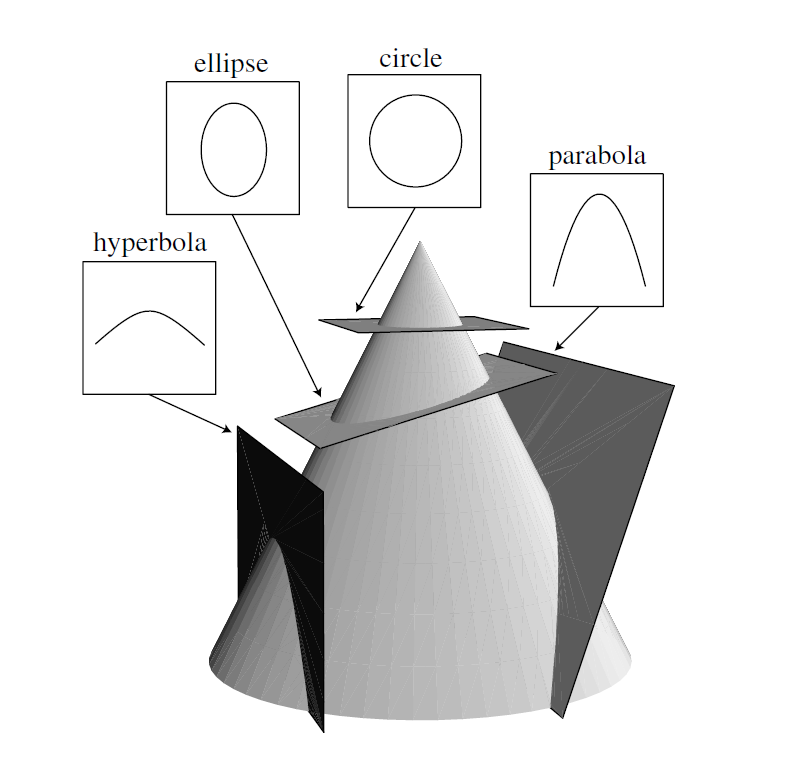
\includegraphics[width=\textwidth]{Pic/Conics.png}
\caption{\cite{murray1999solar}}
\label{Area_dynamics}
\end{center}
\end{figure}

\end{columns}
\end{frame}

\begin{frame}{Celestial mechanics \cite{murray1999solar}: $3^{th}$ Kepler law}
\begin{columns}
\column{0.4\textwidth}

\begin{figure}[h]
\begin{center}
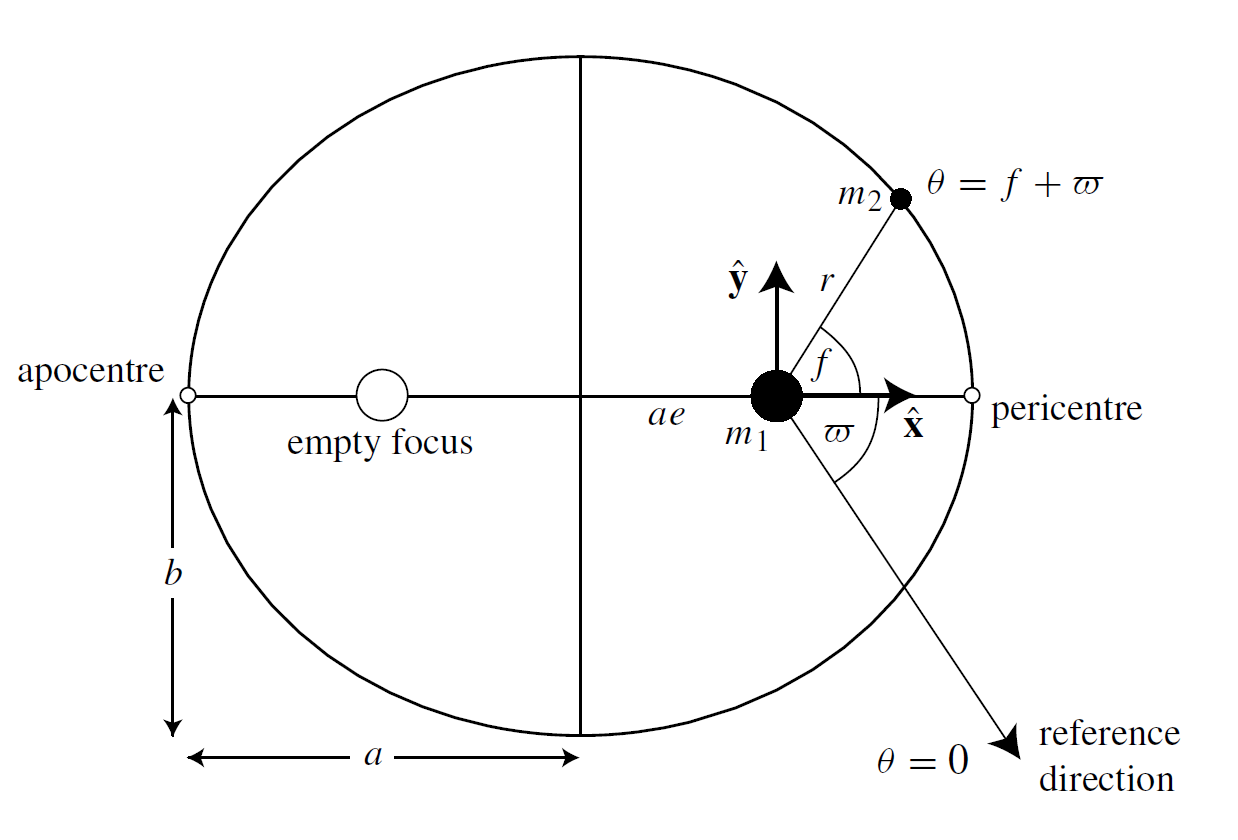
\includegraphics[width=\textwidth ]{Pic/Elliptical_orbit.png}
\caption{\cite{murray1999solar}}
\label{Area_dynamics}
\end{center}
\end{figure}


\column{0.6\textwidth}
\begin{equation}
b^{2}=a^{2}(1-e^{2})
\end{equation}


\begin{equation}
r=\frac{a(1-e^{2})}{1+e\cdot cos(\theta-\phi)}
\label{eq-mot}
\end{equation}

\begin{center}
Area swept in one \textcolor{red}{orbital period} T 
\end{center} 
\begin{center}
$A=\pi ab$
\end{center} 
\begin{center}
We know that: $hT/2 \quad h^{2}=\mu a(1-e^{2})$ 
\end{center}
\begin{center}
Therefore 
\end{center}
\begin{equation}
T^{2}=\dfrac{4\pi^{2}}{\mu}a^{3}
\end{equation}

\end{columns}
\end{frame}

\begin{frame}{Celestial mechanics \cite{murray1999solar}: $3^{th}$ Kepler law}


\begin{equation}
\frac{m_{c}+m}{m_{c}+m'}=\left(\frac{a}{a'}\right)^{3}\left(\frac{T'}{T}\right)^{2}
\end{equation}

But since $m$,$m'<<m_{c}$

\begin{equation}
\left(\frac{a}{a'}\right)^{3}\approx \left(\frac{T}{T'}'\right)^{2}
\end{equation}

And therefore 

\begin{equation}
T'\approx a'^{3/2}
\end{equation}

\begin{center}
\textbf{Remark:} The mass of the asteroid is \textbf{not} involved
\end{center}


\end{frame}

\begin{frame}{Celestial mechanics \cite{murray1999solar}: Orbital parameters}
\begin{center}
\textcolor{red}{Mean motion} $n=\frac{2\pi}{T}$
\end{center}

\begin{equation}
v_{perihelion}=na\sqrt{\dfrac{1+e}{1-e}}
\end{equation}

\begin{equation}
v_{aphelion}=na\sqrt{\dfrac{1-e}{1+e}}
\end{equation}

\begin{center}
\textbf{Remark:} The mean motion of an asteroid is different with respect to the the asteroid relative velocity (measured from Earth), since the latter is different at the perihelion an at the aphelion
\end{center}



\end{frame}



\begin{frame}{Celestial mechanics \cite{murray1999solar}: Orbital parameters}
\begin{columns}
\column{0.4\textwidth}
\begin{figure}[h]
\begin{center}
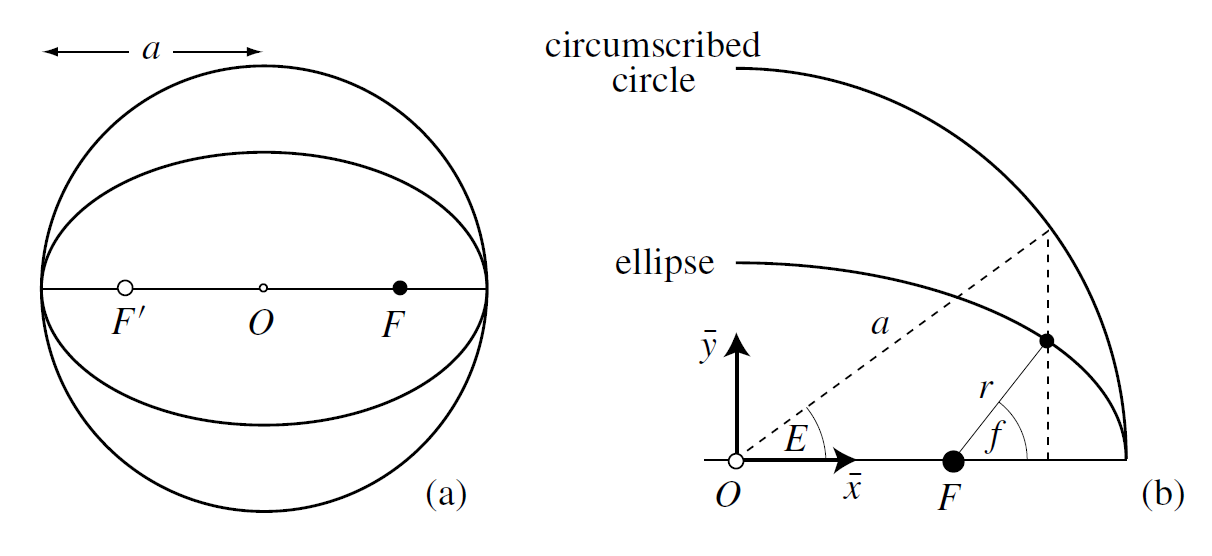
\includegraphics[width=\textwidth ]{Pic/Mean_anomaly.png}
\caption{\cite{murray1999solar}}
\label{Area_dynamics}
\end{center}
\end{figure}
\column{0.6\textwidth}
\begin{center}
\textcolor{red}{Mean anomaly}
\end{center}
\begin{equation}
M=n(t-\tau)
\end{equation}

\begin{center}
\begin{itemize}
\item $M=f=0$\quad$t=\tau$\quad Perihelion
\item $M=f=\pi$\quad$t=\tau+T/2$ \quad Aphelion
\end{itemize}
\end{center}

\begin{equation}
M=E-e\sin E
\end{equation}
\begin{center}
\textcolor{red}{Jupiter Tisserard invariant }
\end{center}
\begin{equation}
T_{P}=\frac{a_{p}}{a}+2\cos I\sqrt{\dfrac{a}{a_{p}}(1-e^{2})}
\end{equation}
\end{columns}
\end{frame}


\begin{frame}{Celestial mechanics \cite{murray1999solar}: Orbital parameters}

\begin{figure}[h]
\begin{center}
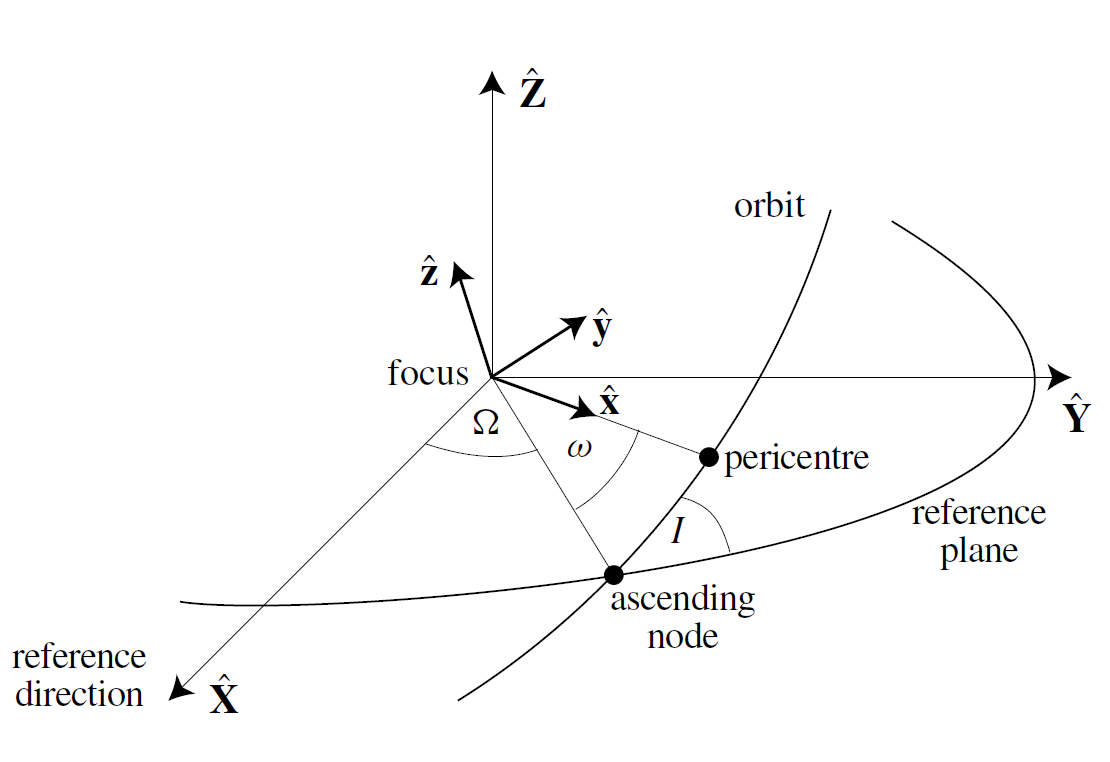
\includegraphics[width=0.6\textwidth ]{Pic/Inclination.png}
\caption{\cite{murray1999solar}}
\label{Area_dynamics}
\end{center}
\end{figure}

\begin{center}
I: \textcolor{red}{inclination} of the orbit
\end{center}
\begin{center}
$\Omega$: \textcolor{red}{longitude of the ascending node}
\end{center}
\end{frame}

\begin{frame}{Celestial mechanics \cite{murray1999solar}: Magnitude}
\begin{equation}
\Phi=\frac{L}{4\pi r^{2}}
\end{equation}
\begin{equation}
m=-2.5\log_{10}\Phi+C
\end{equation}
\begin{equation}
m_{1}-m_{2}=-2.5\log_{10}\frac{\Phi_{1}}{\Phi_{2}}
\end{equation}
\begin{equation}
M-m=-2.5\log_{10}\frac{\Phi\cdot d^{2} }{\Phi\cdot 10^{2}}
\end{equation}
\begin{equation}
M=m+5-5log_{10}d
\end{equation}
Where $\Phi$ is the flux for a sphere of radius r, m the relative magnitude and M the \textcolor{red}{Absolute magnitude}
\end{frame}

\begin{frame}{Celestial mechanics \cite{murray1999solar}: Magnitude}
\begin{equation}
\Phi=\frac{L}{4\pi r^{2}}
\end{equation}
\begin{equation}
m=-2.5\log_{10}\Phi+C
\end{equation}
\begin{equation}
m_{1}-m_{2}=-2.5\log_{10}\frac{\Phi_{1}}{\Phi_{2}}
\end{equation}
\begin{equation}
M-m=-2.5\log_{10}\frac{\Phi\cdot d^{2} }{\Phi\cdot 10^{2}}
\end{equation}
\begin{equation}
M=m+5-5log_{10}d
\end{equation}
Where $\Phi$ is the flux for a sphere of radius r, m the relative magnitude and M the \textcolor{red}{Absolute magnitude}
\end{frame}

\begin{frame}{Celestial mechanics \cite{nasa_classification}: Classification}
\begin{figure}[h]
\begin{center}
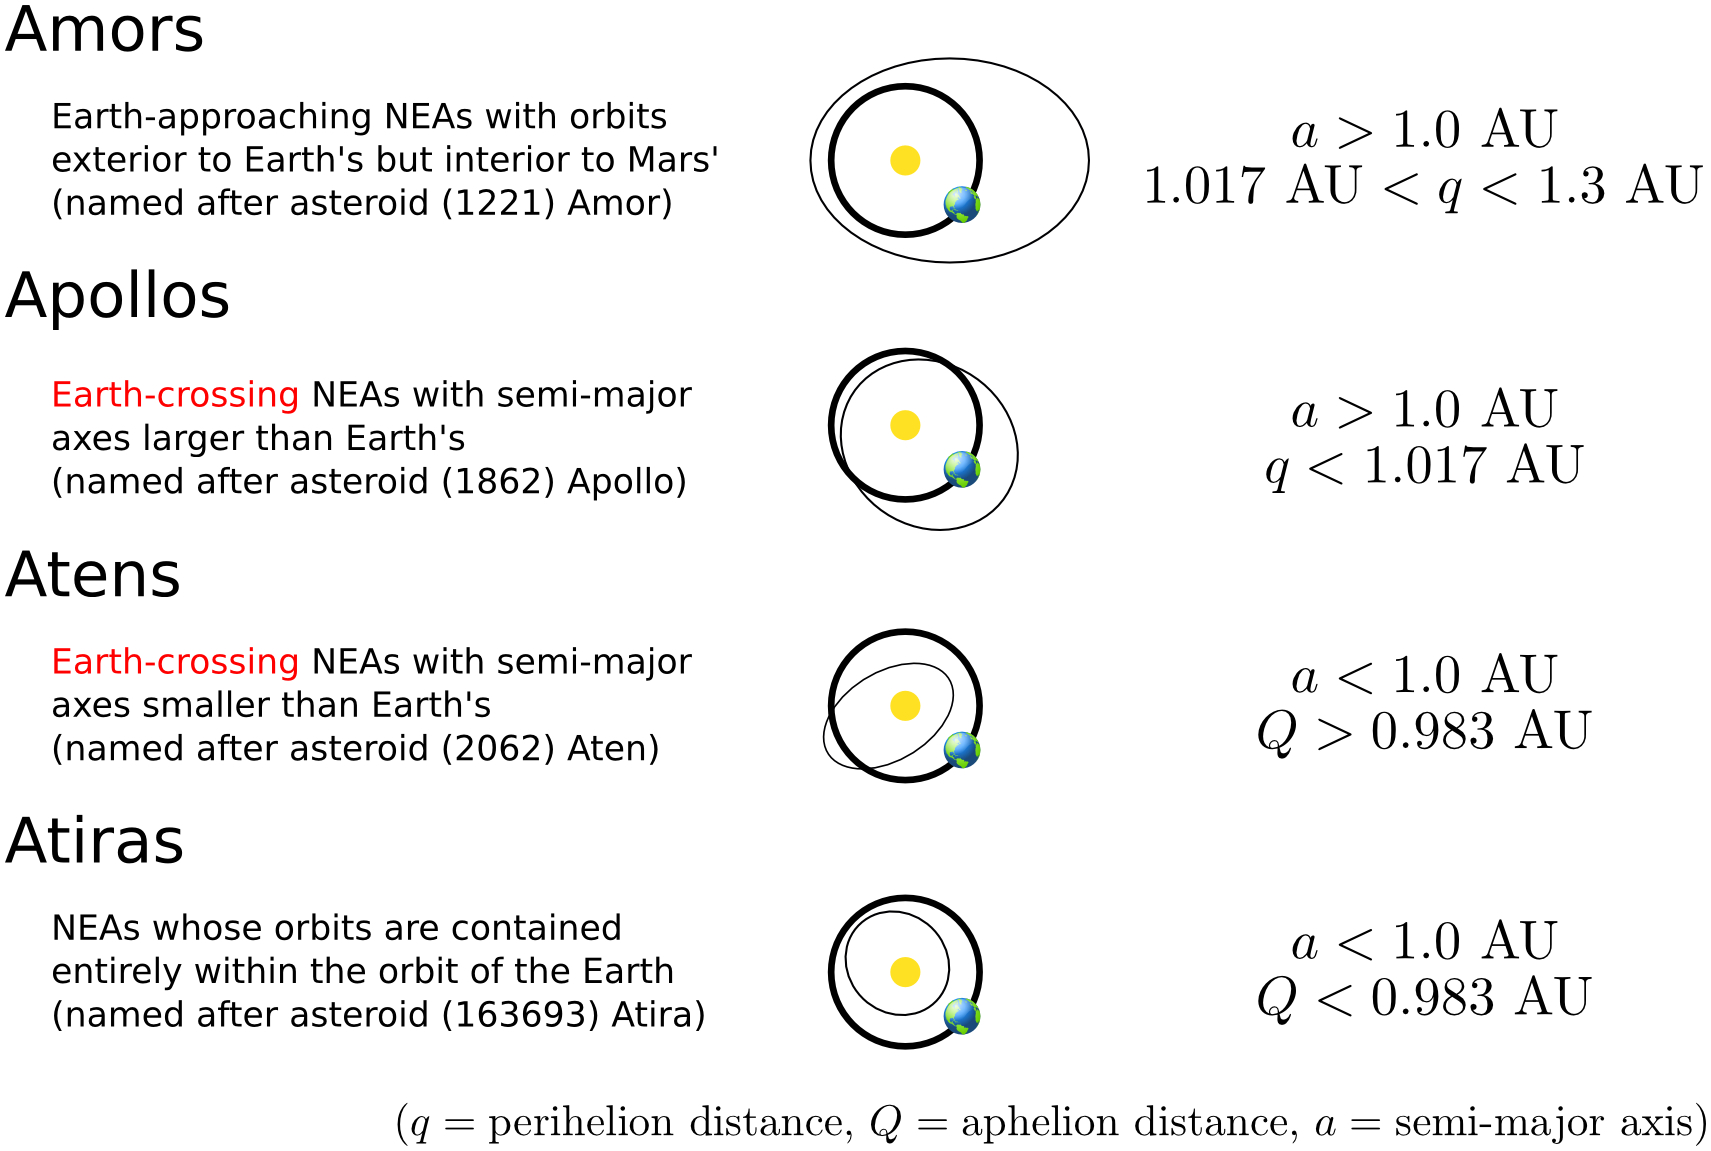
\includegraphics[width=\textwidth]{Pic/neo_orbit_types.jpg}
\caption{\cite{nasa_classification}}
\label{Area_dynamics}
\end{center}
\end{figure}
\end{frame}

\begin{frame}{Celestial mechanics \cite{nasa_classification}: Classification}
\begin{itemize}
\item \textbf{Potentially Hazardous Asteroids}: MOID $\leq 0.05$ au $M \leq22.0$ \textit{NEAs whose Minimum Orbit Intersection Distance (MOID) with the Earth is 0.05 au or less and whose absolute magnitude (M) is 22.0 or brighter}
\end{itemize}
\end{frame}

\section{Dataset}

\begin{frame}{Dataset}
\begin{itemize}


\item The asteroid dataset was retrieved from Kaggle \cite{kaggle_dataset}, which reports into a more machine readable form the dataset of The Center for Near-Earth Object Studies (CNEOS) \cite{cneos+nasa}, a NASA research centre.

\item 3552 Asteroids

\item Among the 40 the features, the ones connected only to the other name of
the asteroid, or connected only to the name of the orbit and
the one connected with the orbiting planet ( since for all it was
the Earth) were discarted

\item The proportion hazardous/not hazardous was set 1:5  

\item The continuous measures were standardised and demeaned

\end{itemize}
\end{frame}

\begin{frame}{Features}
\begin{table}[]
\begin{center}
\begin{tabular}{c|c}
\hline
\textbf{Features}             & \textbf{Type}        \\ \hline
Neo Reference ID              & not used             \\ \hline
Absolute Magnitude            & Continuous           \\ \hline
Est Dia in KM (min)           & Continuous           \\ \hline
Est Dia in KM (max)           & Continuous           \\ \hline
Close Approach Date           & Continuous           \\ \hline
Epoch Date Close Approach     & Continuous           \\ \hline
Relative\_Velocity            & Continuous           \\ \hline
Miss\_Dist                    & Continuous           \\ \hline
Min\_Orbit\_Intersection      & Continuous           \\ \hline
Jupiter\_Tisserand\_Invariant & Continuous           \\ \hline
Epoch\_Osculation             & Continuous           \\ \hline
Eccentricity                  & Continuous           \\ \hline

\end{tabular}
\end{center}
\label{tab_features}
\end{table}

\end{frame}


\begin{frame}{Features}
\begin{table}[]
\begin{center}
\begin{tabular}{c|c}
\hline
\textbf{Features}             & \textbf{Type}        \\ \hline
Semi Major Axis               & Continuous           \\ \hline
Inclination                   & Continuous           \\ \hline
Asc Node Longitude            & Continuous           \\ \hline
Orbital Period                & Continuous           \\ \hline
Perihelion Distance           & Continuous           \\ \hline
Perihelion Arg                & Continuous           \\ \hline
Perihelion Time               & Continuous           \\ \hline
Mean\_Anomaly                 & Continuous           \\ \hline
Mean\_Motion                  & Continuous           \\ \hline
Hazardous                     & Categorical (Binary)
\end{tabular}
\end{center}
\label{tab_features}
\end{table}

\end{frame}


\section{Prelim. analysis}

\begin{frame}{Density Plot}
\begin{columns}
\column{0.5\textwidth}
  \begin{figure}[b]{\textwidth}
    \centering
    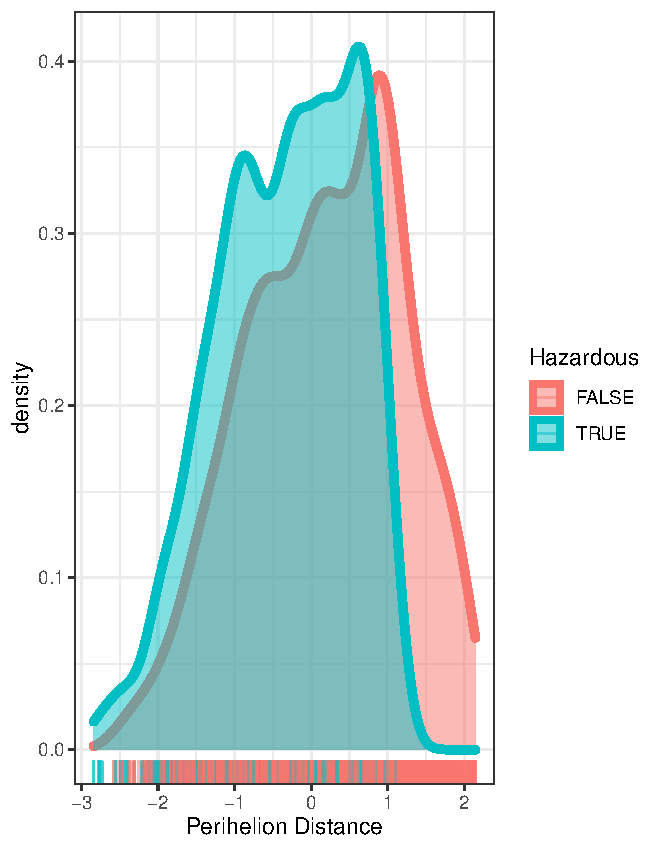
\includegraphics[width=\textwidth]{Pic/DENSITY_Perihelion_Distance.pdf}
    \subcaption{ \begin{center}
    a) Perihelion Distance
    \end{center}}
    \vspace{4ex}
  \end{figure} 
\column{0.5\textwidth}
  \begin{figure}[b]{\textwidth}
    \centering
    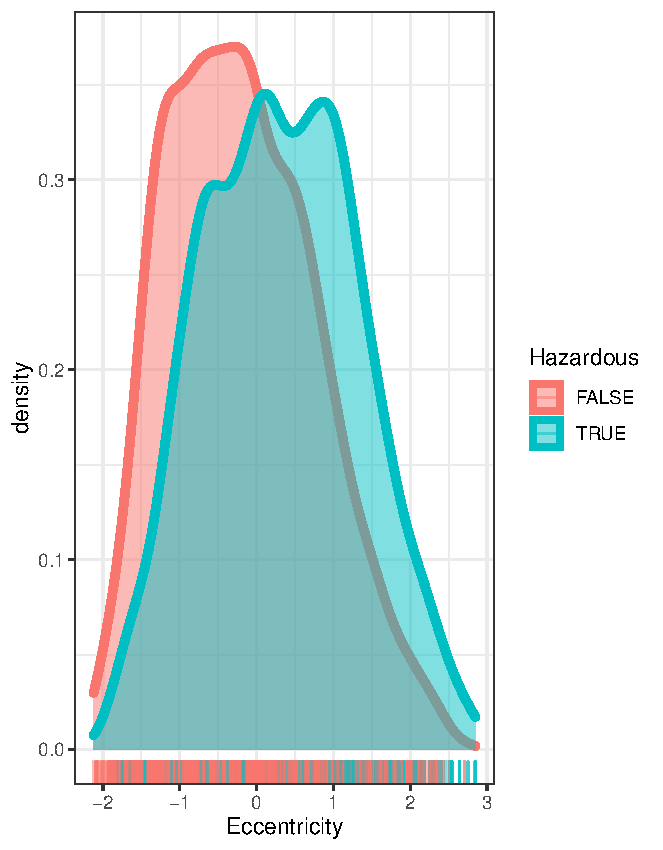
\includegraphics[width=\textwidth]{Pic/DENSITY_Eccentricity.pdf}
    \subcaption{ \begin{center}
    b) Eccentricity
    \end{center}}
    \vspace{4ex}
  \end{figure}
\end{columns}
\end{frame}

\begin{frame}{Density Plot}
\begin{columns}  

\column{0.5\textwidth}
    \begin{figure}[b]{\textwidth}
    \centering
    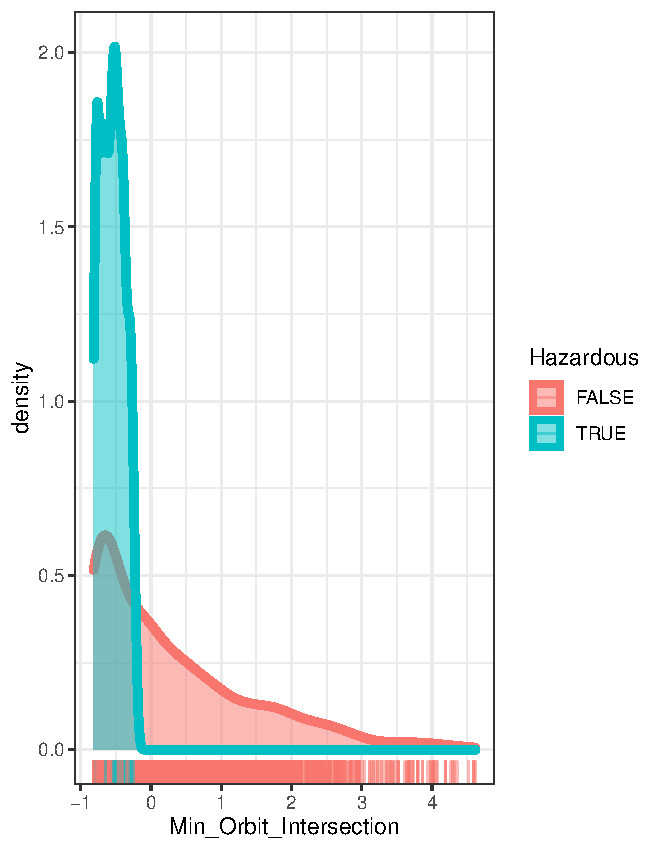
\includegraphics[width=\textwidth]{Pic/DENSITY_Min_orbit_intersection.pdf}
    \subcaption{ \begin{center}
    c) Min orbit intersection
    \end{center}}
    \vspace{4ex}
  \end{figure}
  \column{0.5\textwidth}
  \begin{figure}[b]{\textwidth}
    \centering
    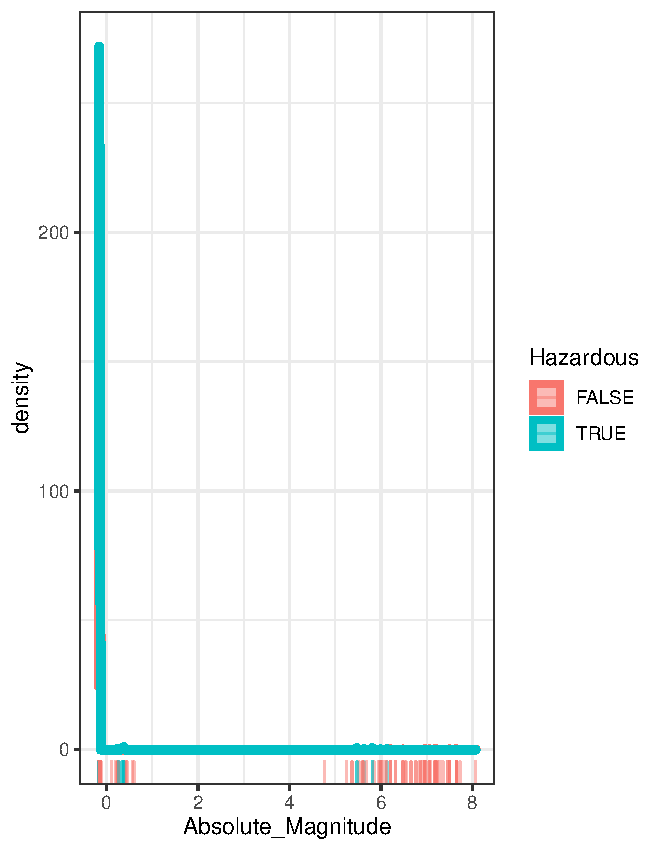
\includegraphics[width=\textwidth]{Pic/DENSITY_Absolute_magnitude.pdf}
    \subcaption{ \begin{center}
    d) Absolute magnitude
    \end{center}}
    \vspace{4ex}
  \end{figure}
\end{columns}
\end{frame}


\begin{frame}{FAMD }
\begin{columns}  

\column{0.5\textwidth}
    \begin{figure}[h]
\begin{center}
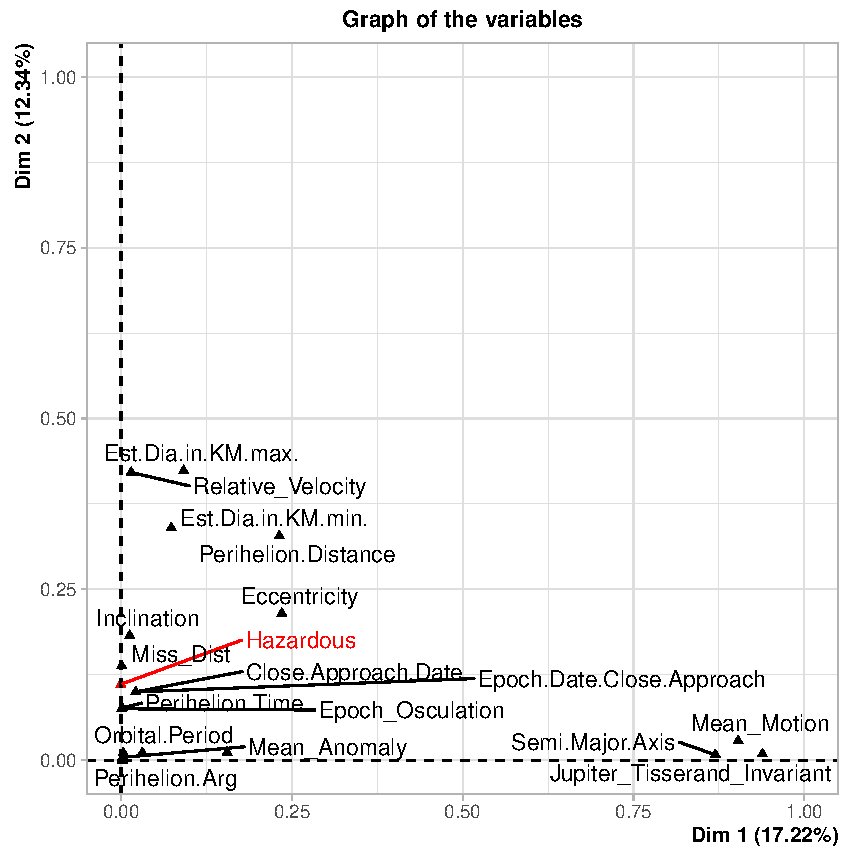
\includegraphics[width=1\textwidth]{Pic/FAMD.pdf}
\label{FADM}
\end{center}
\end{figure}
  \column{0.5\textwidth}
 \begin{figure}[h]
\begin{center}
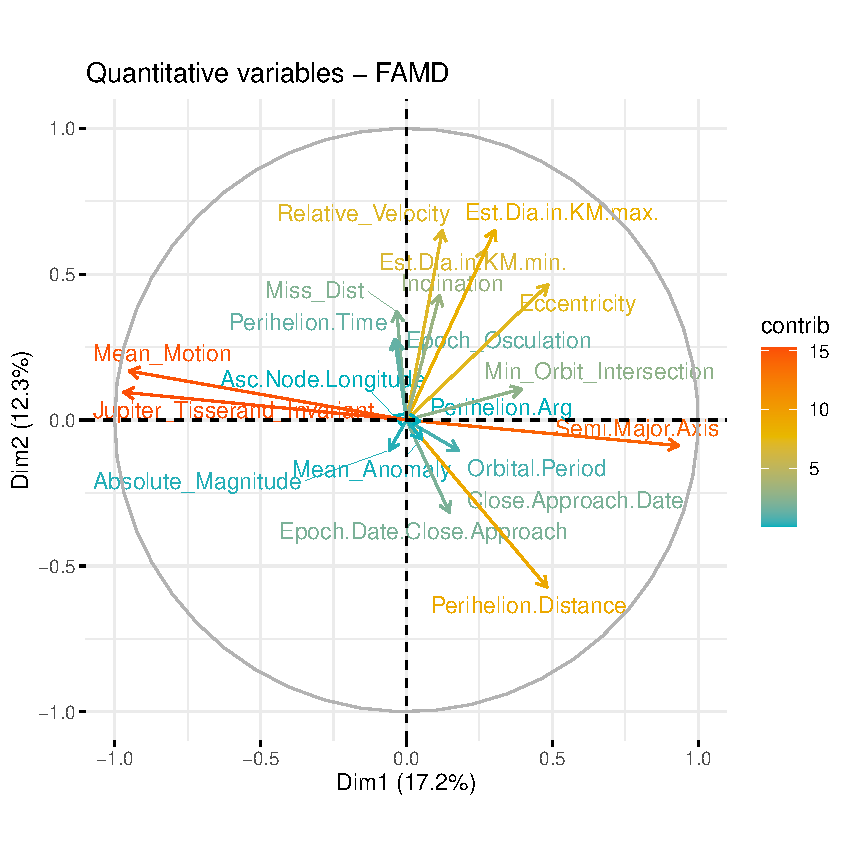
\includegraphics[width=1\textwidth]{Pic/FAMD_Quantitative variables.pdf}
\label{FAMD_Quantitative variables}
\end{center}
\end{figure}
\end{columns}
\begin{center}
Performed with the FactoMineR package \cite{le2008factominer} 
\end{center}
\end{frame}

\begin{frame}{Mutual information analysis}
\begin{figure}
\begin{center}
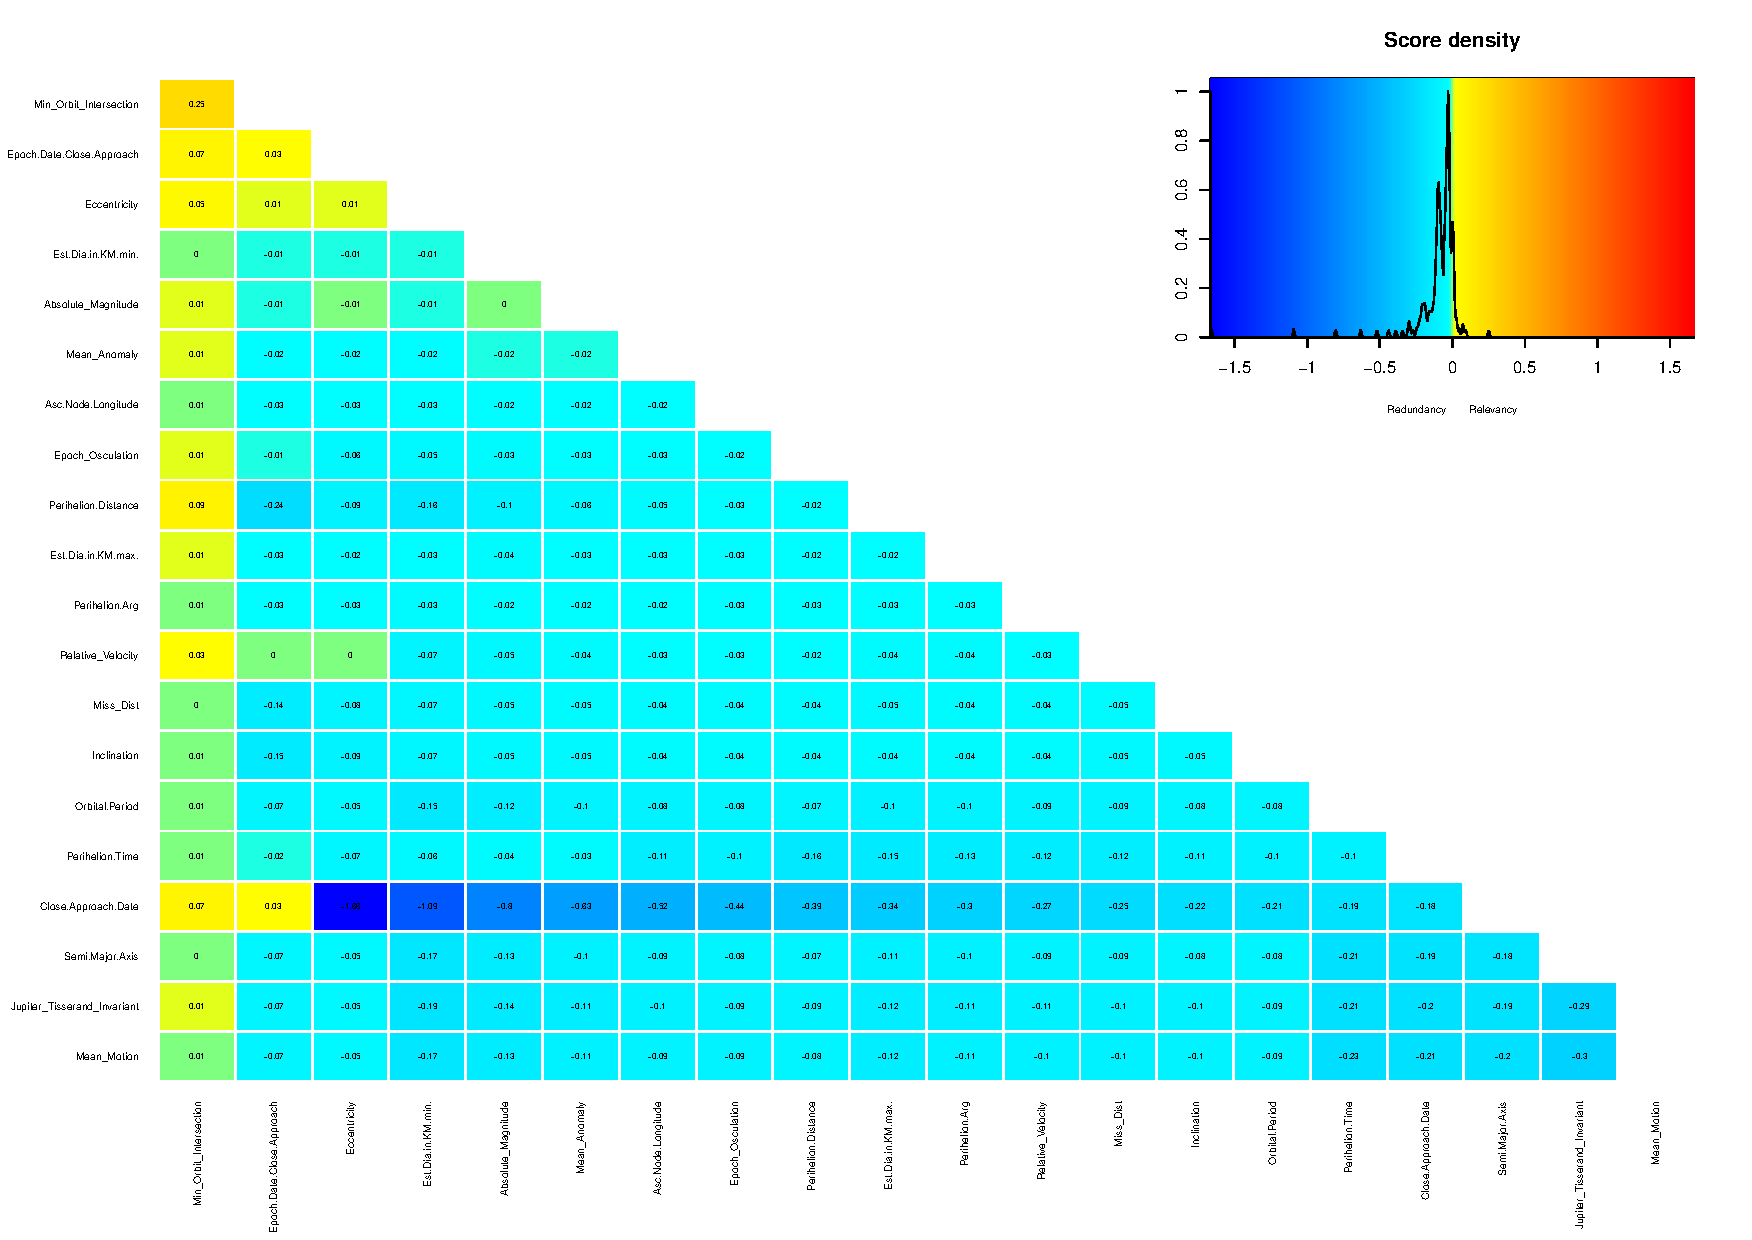
\includegraphics[width=0.8\textwidth]{Pic/Mutual_information.pdf}
\label{Mutual_information}
\end{center}
\end{figure}
\begin{center}
Performed with the varrank package \cite{kratzer2018varrank} 
\end{center}
\end{frame}

\section{Prob. mod.}

\begin{frame}{GLASSO}
\begin{columns}
\column{0.5\textwidth}
  \begin{figure}[b]{\textwidth}
    \centering
    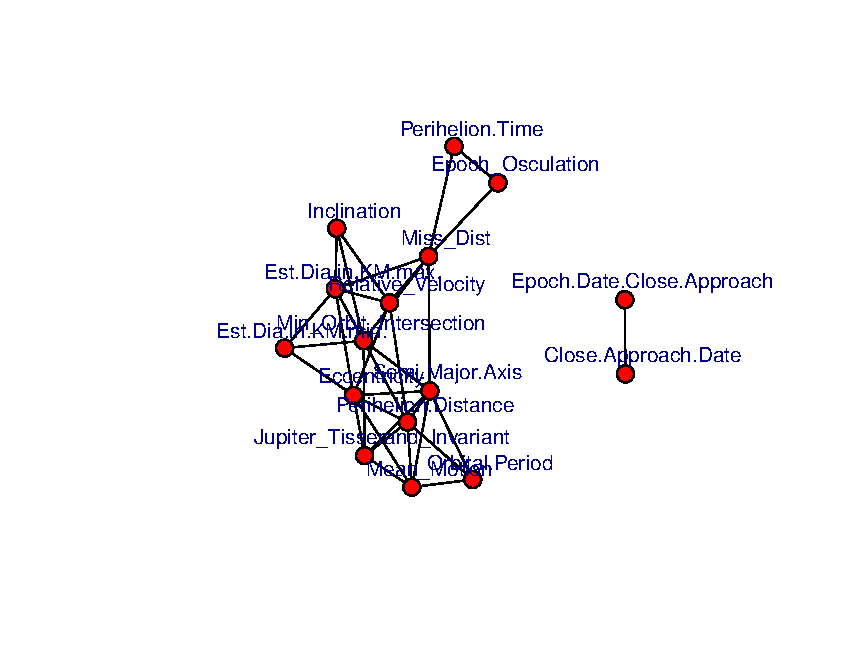
\includegraphics[width=\textwidth]{Pic/GLASSO_0.1.pdf}
    \subcaption{$\rho$=0.2 \begin{center}
    \end{center}}
  \end{figure} 
  \column{0.5\textwidth}
  \begin{figure}[b]{\textwidth}
    \centering
    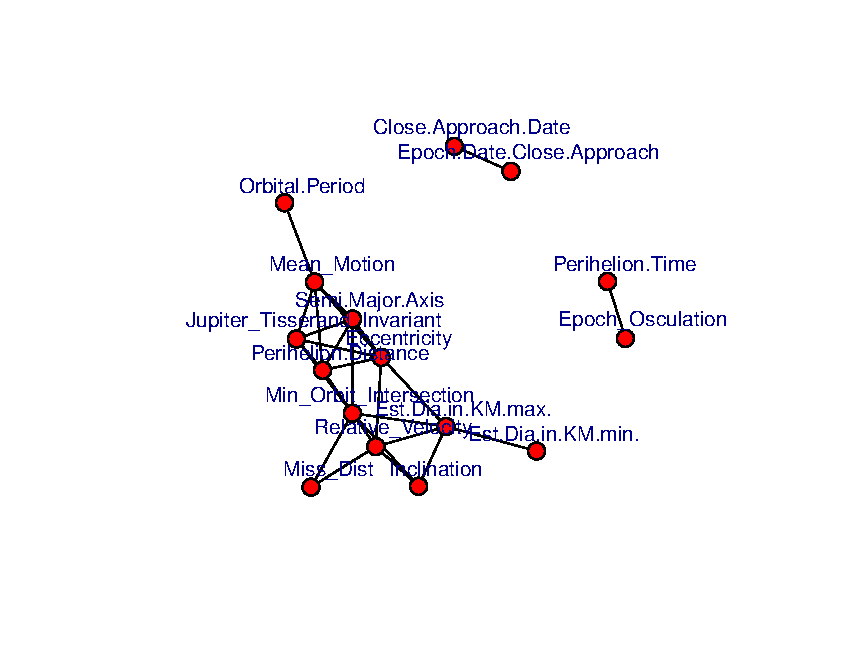
\includegraphics[width=\textwidth]{Pic/GLASSO_0.2.pdf}
    \subcaption{$\rho$=0.2 \begin{center}
    \end{center}}
  \end{figure}
\end{columns}
\begin{center}
Performed with the GLASSO package \cite{glasso}
\end{center}
\end{frame}

\begin{frame}{GLASSO}
\begin{columns}
\column{0.5\textwidth}
  \begin{figure}[b]{\textwidth}
    \centering
    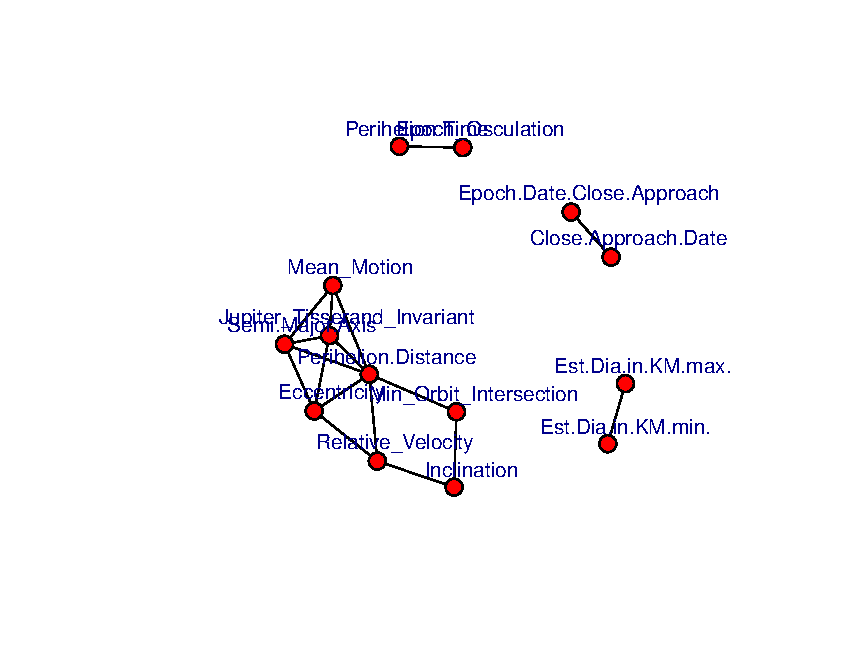
\includegraphics[width=\textwidth]{Pic/GLASSO_0.3.pdf}
    \subcaption{$\rho$=0.3 \begin{center}
    \end{center}}
  \end{figure} 
  \column{0.5\textwidth}
  \begin{figure}[b]{\textwidth}
    \centering
    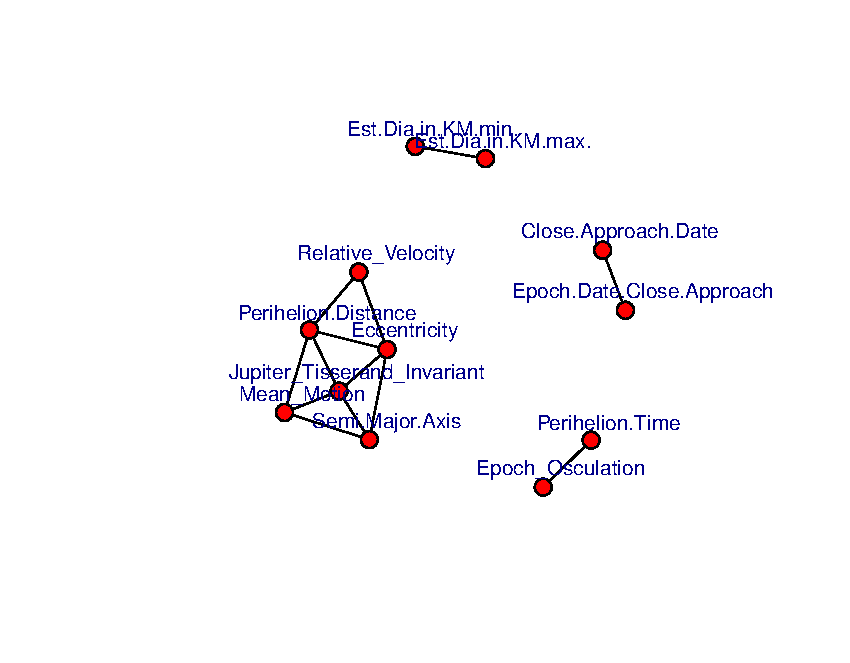
\includegraphics[width=\textwidth]{Pic/GLASSO_0.4.pdf}
    \subcaption{$\rho$=0.4 \begin{center}
    \end{center}}
  \end{figure}
\end{columns}
\begin{center}
Performed with the GLASSO package \cite{glasso}
\end{center}
\end{frame}


\begin{frame}{Mixed interactions: mgm}
\begin{figure}[h]
\begin{center}
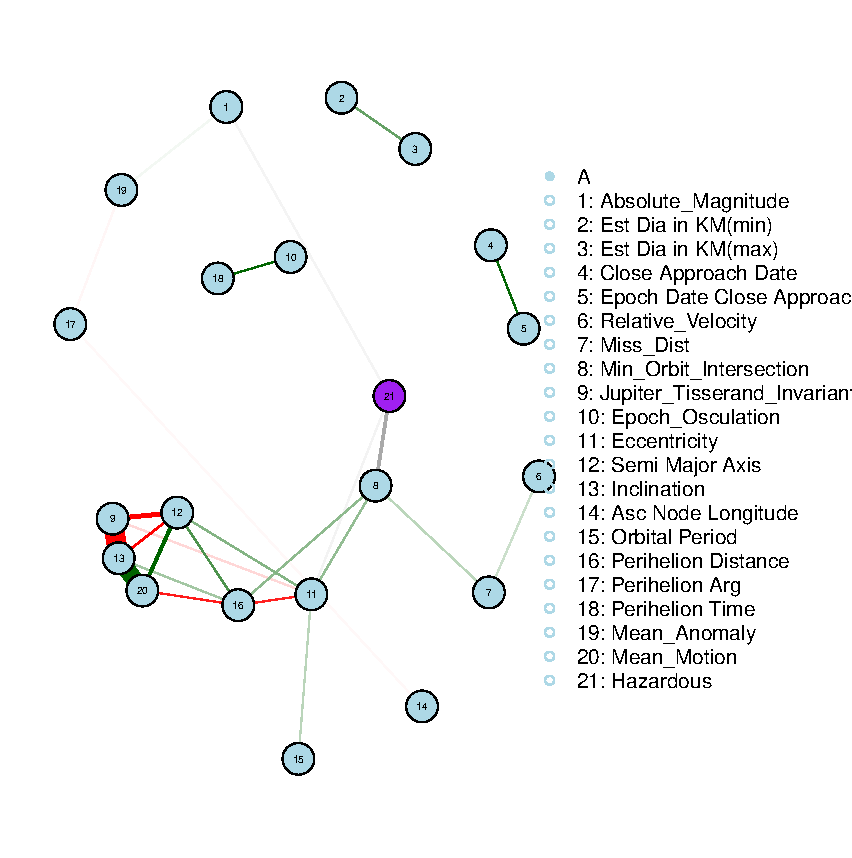
\includegraphics[width=0.6\textwidth]{Pic/mgm.pdf}
\label{mgm}
\end{center}
\end{figure}
\begin{center}
Performed with the mgm package \cite{haslbeck2015mgm}
\end{center}
\end{frame}

\begin{frame}{Mixed interactions: minforest}
\begin{figure}[h]
\begin{center}
\includegraphics[width=0.6\textwidth]{Pic/minforest.pdf}
\label{mgm}
\end{center}
\end{figure}
\begin{center}
Performed with the gRapHD package \cite{de2009high}
\end{center}
\end{frame}

\begin{frame}{Mixed interactions: mmod}
\begin{figure}[h]
\begin{center}
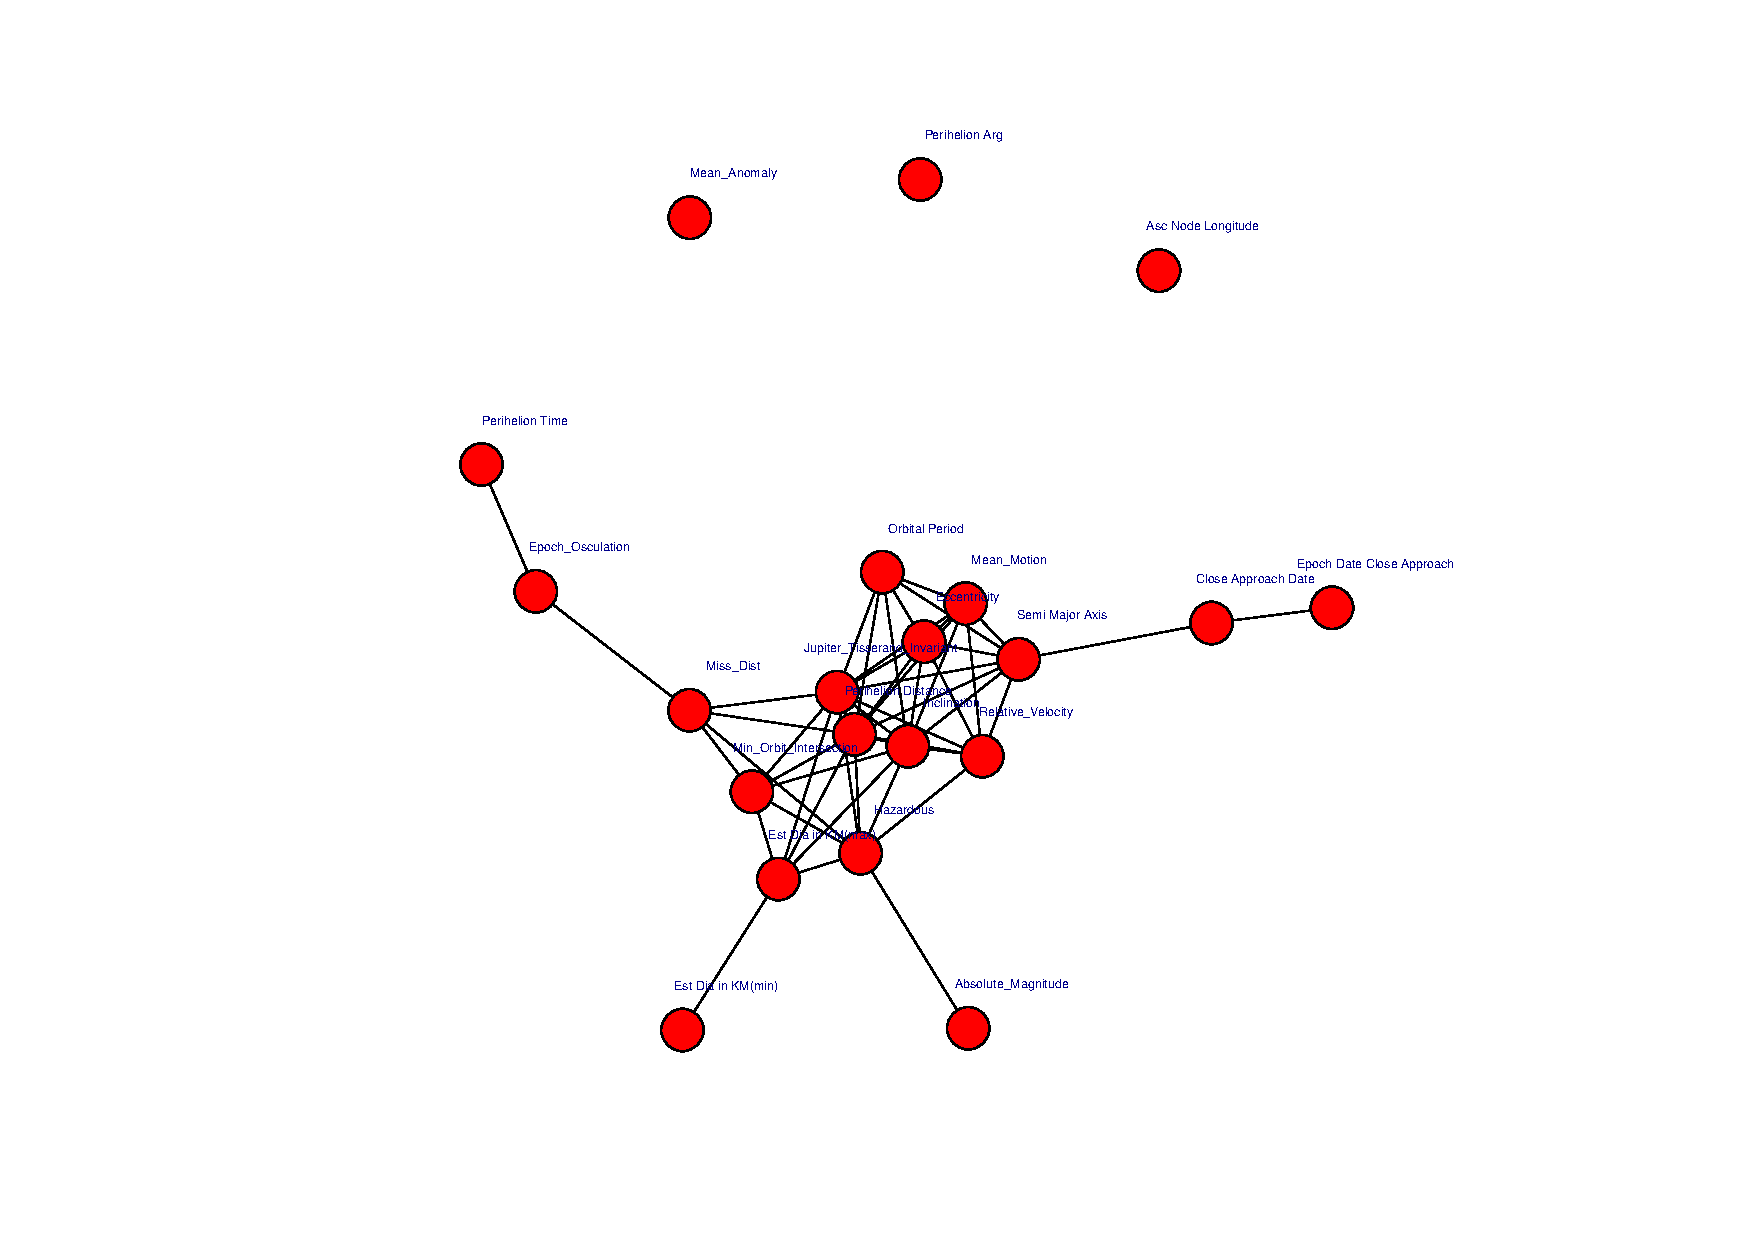
\includegraphics[width=0.6\textwidth]{Pic/mmod.pdf}
\label{mgm}
\end{center}
\end{figure}
\begin{center}
Performed with the gRim package \cite{grim}
\end{center}
\end{frame}

\begin{frame}{Mixed interactions}
The mgm model is the one that has the list of connection more coherent with the celestial mechanics laws. 
\begin{columns}
\column{0.5\textwidth}
  \begin{figure}[b]{\textwidth}
    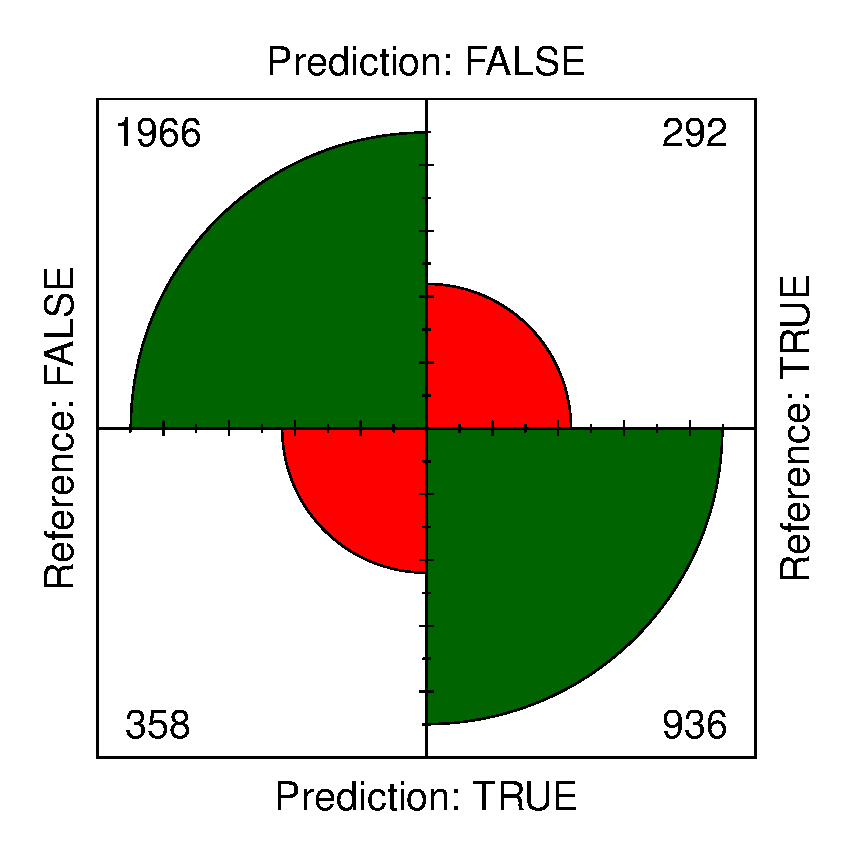
\includegraphics[width=\textwidth]{Pic/mgm_confusion.pdf}
  \end{figure} 
  \column{0.5\textwidth}
  \begin{figure}[b]{\textwidth}
    \includegraphics[width=\textwidth]{Pic/ROC_mgm.pdf}
  \end{figure}
\end{columns}
\end{frame}



\section{Other ML alg.}
\begin{frame}{Random Forest}
\begin{columns}
\column{0.5\textwidth}
  \begin{figure}[b]{\textwidth}
    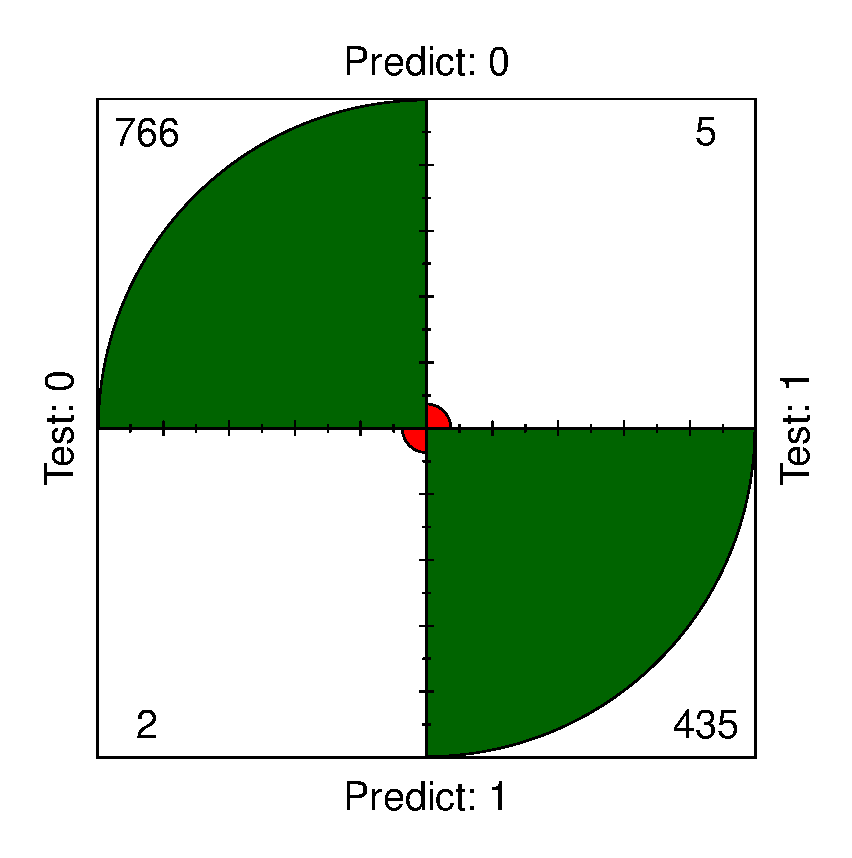
\includegraphics[width=\textwidth]{Pic/RF_confusion.pdf}
  \end{figure} 
  \column{0.5\textwidth}
  \begin{figure}[b]{\textwidth}
    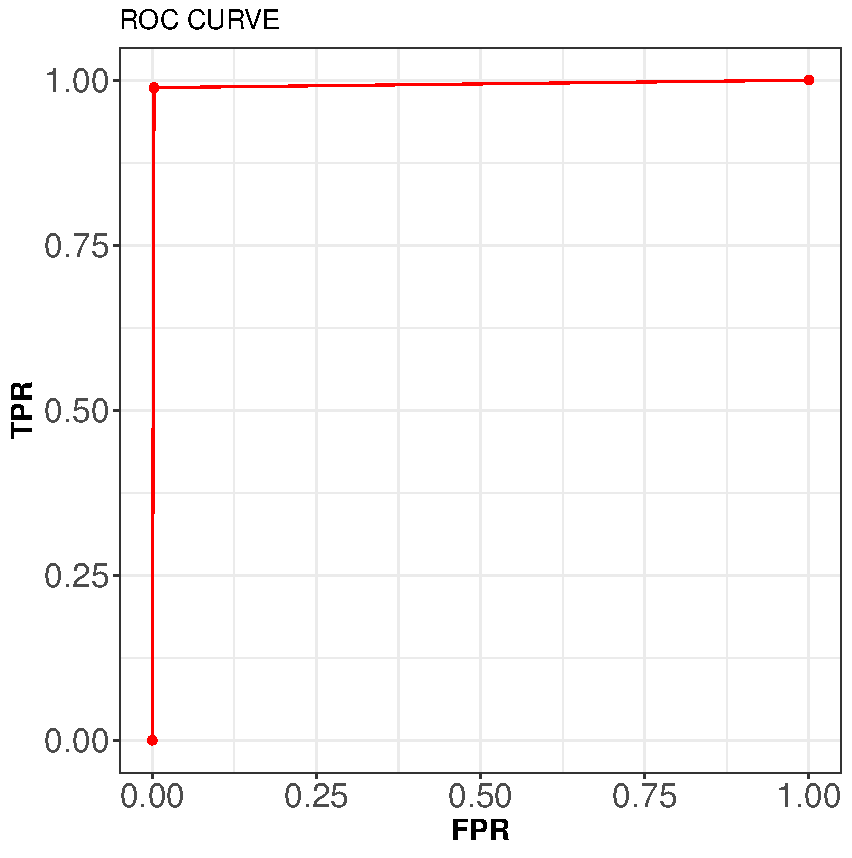
\includegraphics[width=\textwidth]{Pic/ROC_RF.pdf}
  \end{figure}
\end{columns}
\begin{center}
Performed with the rfor package \cite{rfor}
\end{center}
\end{frame}

\begin{frame}{Random Forest}
  \begin{figure}[b]{\textwidth}
    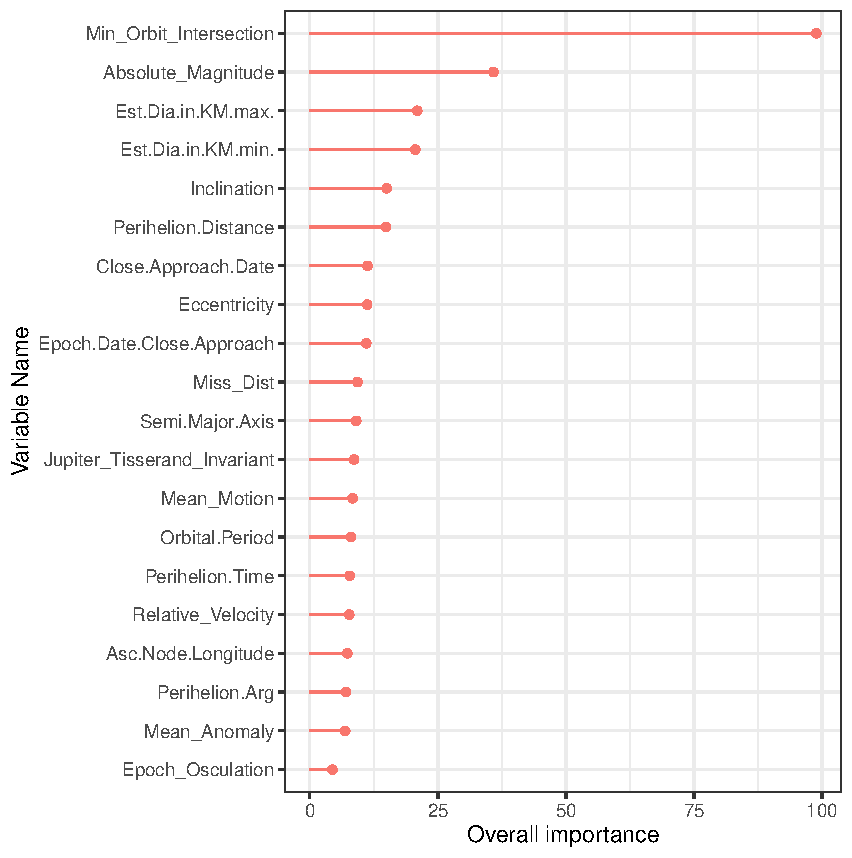
\includegraphics[width=0.7\textwidth]{Pic/RF_Importance.pdf}
  \end{figure} 
\end{frame}

\begin{frame}{Support Vector Machines}
\begin{columns}
\column{0.5\textwidth}
  \begin{figure}[b]{\textwidth}
    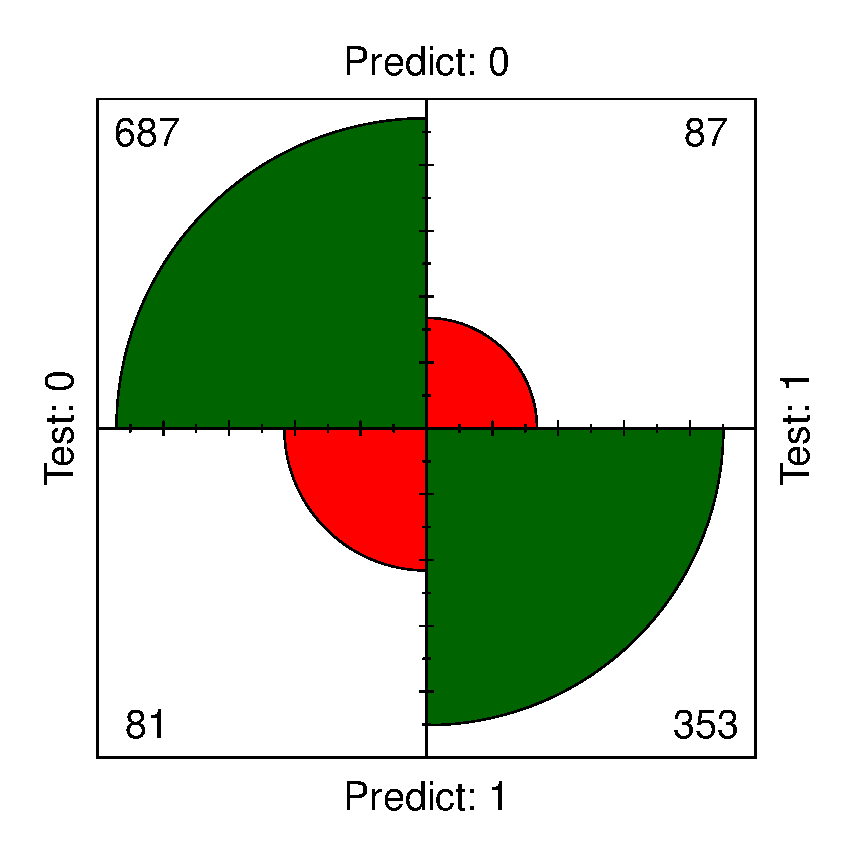
\includegraphics[width=\textwidth]{Pic/SVM_confusion.pdf}
  \end{figure} 
  \column{0.5\textwidth}
  \begin{figure}[b]{\textwidth}
    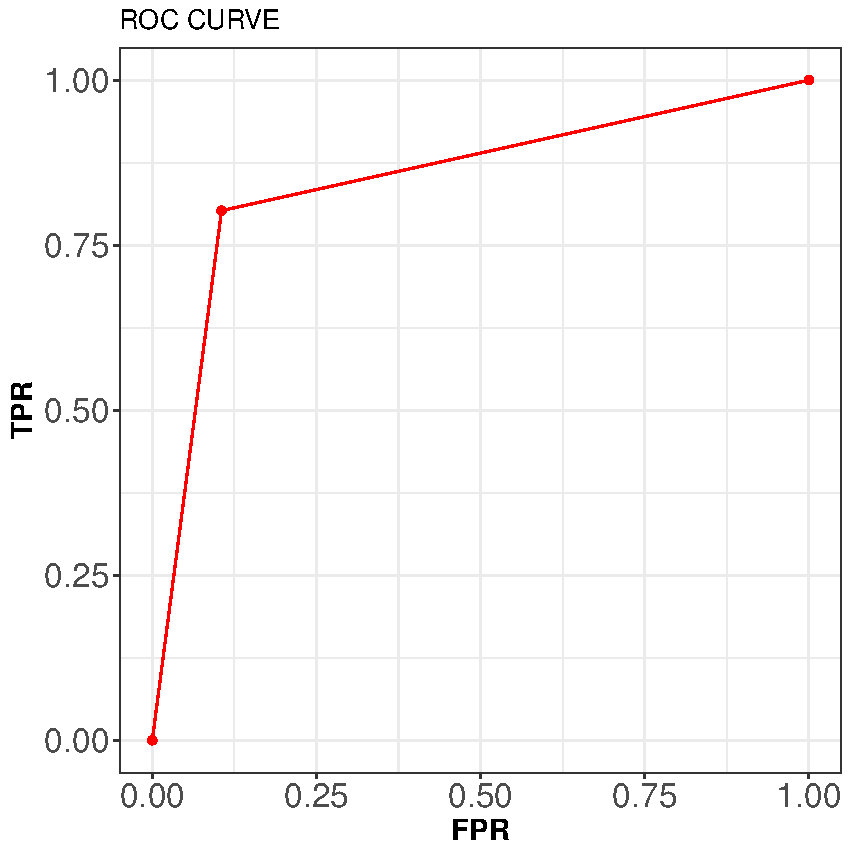
\includegraphics[width=\textwidth]{Pic/ROC_SVM.pdf}
  \end{figure}
\end{columns}
\begin{center}
Performed with the e1071 package \cite{dimitriadou2008misc}
\end{center}
\end{frame}

\begin{frame}{Quadratic Discriminant Analysis (QDA)}
\begin{columns}
\column{0.5\textwidth}
  \begin{figure}[b]{\textwidth}
    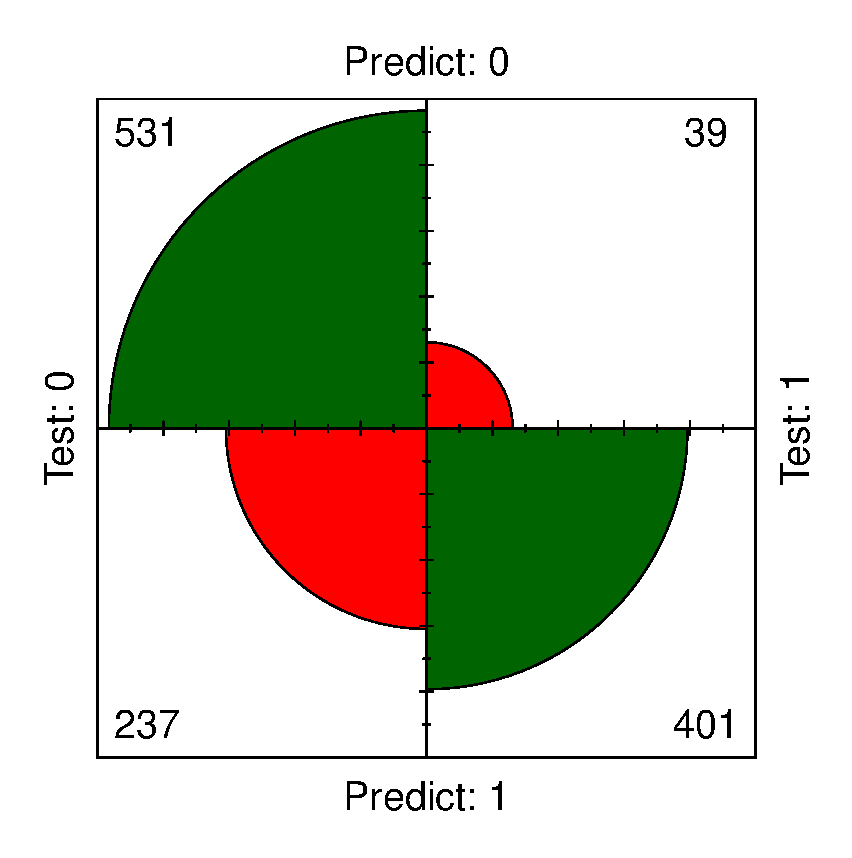
\includegraphics[width=\textwidth]{Pic/QDA_confusion.pdf}
  \end{figure} 
  \column{0.5\textwidth}
  \begin{figure}[b]{\textwidth}
    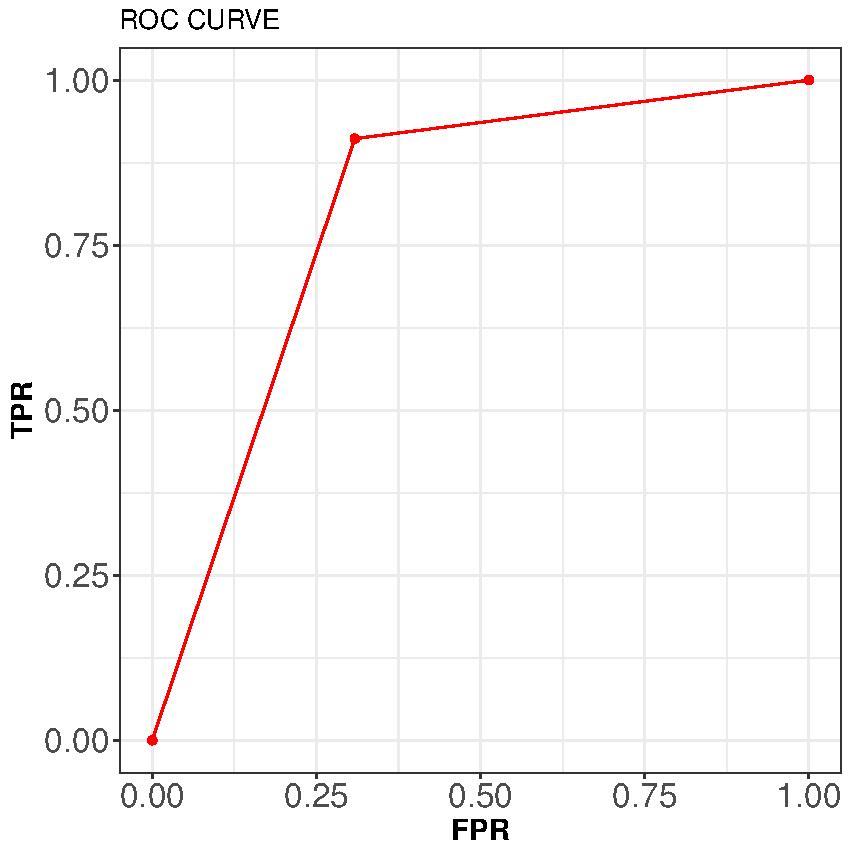
\includegraphics[width=\textwidth]{Pic/ROC_QDA.pdf}
  \end{figure}
\end{columns}
\begin{center}
Performed with the MASS package \cite{MASS}
\end{center}
\end{frame}

\begin{frame}{Logistic regression}
\begin{columns}
\column{0.5\textwidth}
  \begin{figure}[b]{\textwidth}
    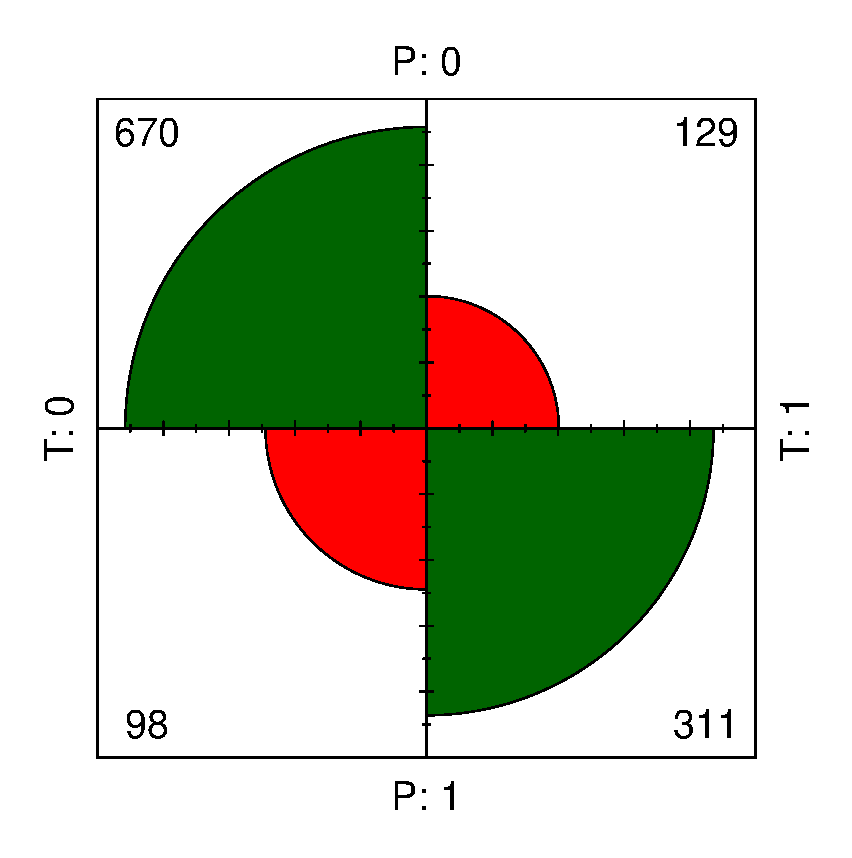
\includegraphics[width=\textwidth]{Pic/Logisic_confusion.pdf}
  \end{figure} 
  \column{0.5\textwidth}
  \begin{figure}[b]{\textwidth}
    \includegraphics[width=\textwidth]{Pic/ROC_Logistic.pdf}
  \end{figure}
\end{columns}
\begin{center}
Performed with the stats package \cite{stats}
\end{center}
\end{frame}




\begin{frame}{$\phi$ coefficient}
\begin{table}[]
\caption{$\phi$ coefficient (also known as Matthews correlation coefficient )}
\begin{center}
\begin{tabular}{c|c}
Algorithm & $\phi$ \\ \hline
RF        & 0.9876 \\ \hline
SVM       & 0.7111 \\ \hline
logistic  & 0.6173 \\ \hline
mgm       & 0.5997 \\ \hline
QDA       & 0.5562 
\end{tabular}
\end{center}
\label{phi_values}
\end{table}
\end{frame}

\section{Conclusions}

\begin{frame}{Interpretability and scientific validation}

\begin{remark}[Interpretability - Tarski definition]
The formal theory T can be translated into S if and only if S can prove the theorem of T in its language \cite{tarski1953undecidable}
\end{remark}

\end{frame}

\begin{frame}{Interpretability and scientific validation}

\begin{remark}[Scientific method - Einstein definition]
Science uses the totality of the primary concepts, i.e., concepts directly connected with sense experiences, and propositions connecting them. Such a state of affairs cannot, however, satisfy a spirit which is really scientifically minded; because the totality of concepts and relations obtained in this manner is utterly lacking in logical unity. In order to supplement this deficiency, one invents a system poorer in concepts and relations, a system retaining the primary concepts and relations of the \textit{first layer} as logically derived concepts and relations. This new \textit{secondary system} pays for its higher logical unity by having elementary concepts (concepts of the second layer), which are no longer directly connected with complexes of sense experiences \cite{physics-reality}
\end{remark}

\end{frame}


\begin{frame}{Interpretability and scientific validation}

\begin{remark}[Scientific method - Einstein definition ]
The essential thing is the aim to represent the multitude of concepts and propositions, close to experience, as propositions, logically deduced from a basis, as narrow as possible, of fundamental concepts and fundamental relations which themselves can be chosen freely (axioms) \cite{physics-reality}
\end{remark}

\end{frame}


\begin{frame}{Conclusions: forecast performances vs intepretability}
\begin{itemize}
\item The mgm algorithm is not the best one in term of performances, but it provides the connections between the features. On the other side, except for the variable importance in RF, the other are black box one
\item The mgm model, as the other graphical model is open to a true scientific validation, the other not. 
\item The probabilistic models lack in the forecast is definitely compensated by their interetability 
\item This is meaningful since this two features are in conflict 
\item The probabilistic models provide a good trade-off between intepretability and forecast performances, as long as one is interest to produce a really scientific result (e.g if the only aim is the forecast the RF is definitely better. However how long one can trust to the RF result ?)
\end{itemize}
\end{frame}

\section{SI}

\begin{frame}
\begin{center}
\frametitle{$\phi$ coefficent}
\begin{table}[]
\begin{tabular}{c|c|c}
\multicolumn{1}{l|}{\textbf{}} & \textbf{Actual - N} & \textbf{Actual - P} \\ \hline
\textbf{Predicted - N}         & \#TP                & \#FN                \\ \hline
\textbf{Predicted - P}         & \#FP                & \#TP               
\end{tabular}
\end{table}
\begin{equation*}
\phi=\dfrac{TP\times TN - FP\times FN}{\sqrt{\left(TP+FP\right)\left(TP+FN\right)\left(TN+FP\right)\left(TN+FN\right)}}
\end{equation*}
\end{center}
\end{frame}

\begin{frame}
\frametitle{Receiver operating characteristic}
\begin{columns}
\column{0.5\textwidth}
\begin{center}
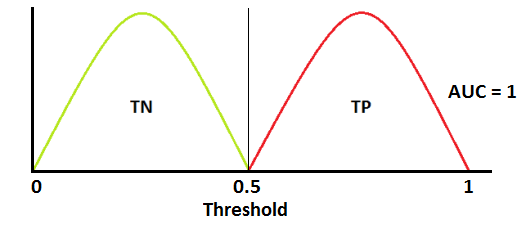
\includegraphics[width=1\linewidth]{Pic/ROC/ROC_A.png}
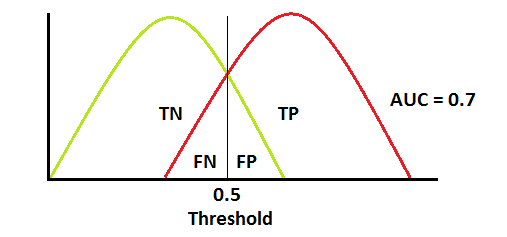
\includegraphics[width=1\linewidth]{Pic/ROC/ROC_B.png}\\
\end{center}
\column{0.5\textwidth}
\begin{center}
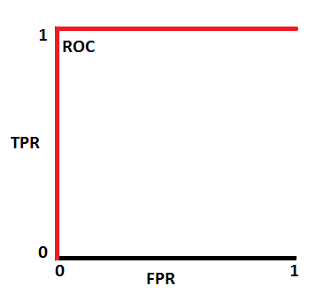
\includegraphics[width=0.5\linewidth]{Pic/ROC/ROC_A_R.png}
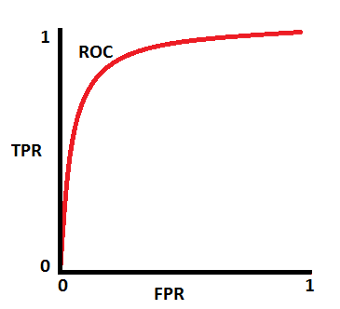
\includegraphics[width=0.5\linewidth]{Pic/ROC/ROC_B_R.png}\\
\end{center}
\end{columns}
\begin{center}
Images taken from \cite{ROC_fig}
\end{center}
\end{frame}


\begin{frame}
\frametitle{Receiver operating characteristic}
\begin{columns}
\column{0.5\textwidth}
\begin{center}
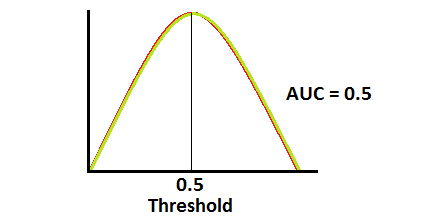
\includegraphics[width=1\linewidth]{Pic/ROC/ROC_C.png}
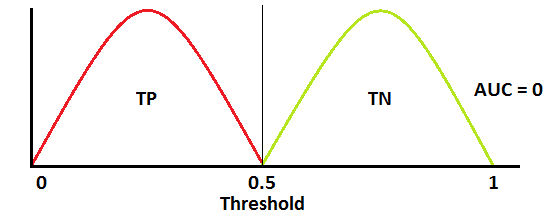
\includegraphics[width=1\linewidth]{Pic/ROC/ROC_D.png}\\
\end{center}
\column{0.5\textwidth}
\begin{center}
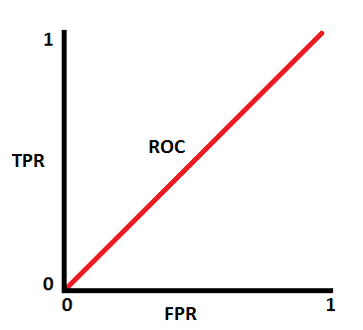
\includegraphics[width=0.5\linewidth]{Pic/ROC/ROC_C_R.png}
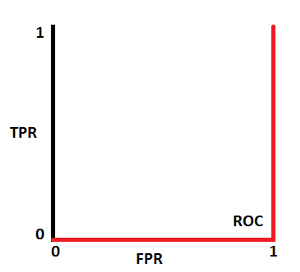
\includegraphics[width=0.5\linewidth]{Pic/ROC/ROC_D_R.png}\\
\end{center}
\end{columns}
\begin{center}
Images taken from \cite{ROC_fig}
\end{center}
\end{frame}


\begin{frame}{Factor analysis of mixed data - FAMD}
\begin{center}
r(z,k) correlation coefficient (z and k quantitative) \\
\end{center}
\begin{center}
$\eta^{2}$(z,q) correlation ratio (z quantitative and q qualitative)
\end{center}
\begin{center}
PCA $\rightarrow$ $max\sum_{k}r^{2}(z,k)$
\end{center}
\begin{center}
MCA $\rightarrow$ $max\sum_{q}\eta^{2}(z,q)$
\end{center}
\begin{center}
FAMD $\rightarrow$ $max\sum_{k}r^{2}(z,k)+max\sum_{q}\eta^{2}(z,q)$
\end{center}
\end{frame}


\begin{frame}{mgm algorithm}
\begin{equation}
P(X_{s}|X_{\backslash s})=\exp\left\lbrace E_{s}(X_{\backslash s})\phi_{s}\left(X_{s}\right)+B_{s}(X_{s})-\Phi\left(X_{\backslash s}\right) \right\rbrace
\end{equation}
\begin{center}
$\phi_{s}$ function of sufficient statistics $B_{s}$ base measure
\end{center}

\begin{equation}
\begin{split}
P(X)= & \exp \left( \sum_{s\in V}\theta_{s}\phi_{s}(X_{s})+\sum_{s\in V}\sum_{r\in N(s)}\theta_{s,r}\phi_{s}(X_{s})\phi_{r}(X_{r})\\ +&...+\sum_{r_{1},...,r_{k}\in C}\theta_{r1,...,rk}\prod_{j=1}^{k}\phi_{r}_{j}\left(X_{r}_{j}\right)+\sum_{s\in V}B_{s}(X_{S})-\Phi(\theta) \right)
\end{split}
\end{equation}

\begin{equation}
\hat{\theta}=arg \min_{theta}\left\lbrace -\mathcal{L}(\theta,X)+\lambda ||\theta ||_{1}  \right\rbrace\quad ||\theta ||_{1}=\sum_{j=1}^{J}|\theta_{j}|
\end{equation}


\end{frame}



\begin{frame}{GLASSO}
\begin{equation}
L_{pen}(K,\hat{\mu})=log\det(K)-tr(K\;S)-\rho||K|| 
\end{equation}
\begin{center}
$K=\Sigma^{-1}$
\end{center}
\begin{center}
S: empirical covariance matrix
\end{center}
\end{frame}

\begin{frame}{Parameters tuning}
\begin{equation}
p\left(\textbf{y}|\boldsymbol{\theta}\right) = \dfrac{1}{Z(\theta)}\exp \left( \sum_{c}\boldsymbol{\theta}^{T}_{c}\phi_{c}\left(\textbf{y}\right)\right)
\end{equation}
\begin{equation}
\mathcal{L}\left(\boldsymbol{\theta}\right):= \frac{1}{N}\sum_{i}\log p\left(\textbf{y}_{i}|\boldsymbol{\theta}\right)=\frac{1}{N}\sum_{i}\left[\sum_{c} \boldsymbol{\theta}^{T}_{c}\phi_{c}(y_{i})-\log Z\left(\boldsymbol{\theta}\right)\right]
\end{equation}
\end{frame}


\begin{frame}{Parameters tuning}
\begin{equation}
\frac{\partial\mathcal{L}}{\partial\boldsymbol{\theta}_{c}}=\frac{1}{N}\sum_{i}\left[\phi_{c}(y_{i})-\frac{\partial}{\partial\boldsymbol{\theta}_{c}}\log Z(\boldsymbol{\theta})\right]
\end{equation}

\begin{equation}
\begin{split}
\frac{\partial \log Z(\boldsymbol{\theta})}{\partial\boldsymbol{\theta}}=\mathbb{E}\left[\phi_{c}(\textbf{y})\right|\theta]= \sum_{\textbf{y}}\phi_{c}(\textbf{y})p(\textbf{y}|\boldsymbol{\theta})
\end{split}
\end{equation}
\begin{equation}
\frac{\partial\mathcal{L}}{\partial\boldsymbol{\theta}_{c}}=\left[\frac{1}{N}\sum_{i}\phi_{c}(y_{i})\right]-\mathbb{E}\left[\phi_{c}(\textbf{y})\right]
\end{equation}
\begin{equation}
\frac{\partial\mathcal{L}}{\partial\boldsymbol{\theta}_{c}}=\mathbb{E}_{p_{emp}}\left[\phi_{c}(\textbf{y})\right]-\mathbb{E}_{p_{(\cdot|\boldsymbol{\theta})}}\left[\phi_{c}(\textbf{y})\right]
\end{equation}
\begin{equation}
\mathbb{E}_{p_{emp}}\left[\phi_{c}(\textbf{y})\right]=\mathbb{E}_{p_{(\cdot|\boldsymbol{\theta})}}\left[\phi_{c}(\textbf{y})\right]
\end{equation}
\end{frame}


\begin{frame}{mmod}
\begin{equation}
\begin{split}
f(i,y)=& p(i)(2\pi)^{-q/2}det(\Sigma)^{-1/2} \\
& exp\left[-\dfrac{1}{2}\left(y-\mu(i)\right)^{T}\Sigma^{-1}\left(y-\mu(i)\right)\right]
\end{split}
\label{gaussMix}
\end{equation}
\begin{equation}
\begin{split}
f(i,y) & = \exp\left\lbrace g(i)+\sum_{u}h^{u}(i)y_{u}-\dfrac{1}{2}\sum_{uv} y_{u}y_{v}k_{uv}\right\rbrace \\
&= \exp\left\lbrace g(i)+h(i)^{T}y-\dfrac{1}{2}y^{T}Ky \right\rbrace
\end{split}
\end{equation}

\begin{center}
where $g(i)$, $h(i)$ and $K$ are the canonical parameters
\end{center}

\end{frame}
\begin{frame}{mmod}
\begin{equation}
\begin{split}
K=&\Sigma^{-1} \\
h(i)=&\Sigma^{-1}\mu(i) \\
g(i)=&\log p(i) -\frac{1}{2}\log det (\Sigma) \\
&-\dfrac{1}{2}\mu(i)^{T}\Sigma^{-1}\mu(i)-\dfrac{q}{2}\log 2\pi
\end{split}
\end{equation}
\end{frame}


\begin{frame}{Graphical models}
\begin{equation}
p(x_{1},x_{2},...,x_{n})
\end{equation}
\begin{equation}
p(x_{1:V})=p(x_{1})p(x_{2}|x_{1})p(x_{3}|x_{2},x_{1})...p(x_{V}|x_{1:V-1})
\end{equation}
\begin{equation}
X  \perp Y| Z \iff  p(X,Y|Z) = p(X|Z)p(Y|Z)
\end{equation}
\begin{equation}
p(\textbf{x}_{1:V})=p(x_{1})\prod^{V}_{t=1}p(x_{t}|x_{t-1})
\end{equation}
\end{frame}


\begin{frame}{Graphical models}
\begin{theorem}[Hammersley-Clifford]
A positive distribution p(\textbf{y})>0 satisfies the CI properties of an indirect graph G iif p can be represented as a product of factor, one per maximal clique,  i.e.
\begin{equation}
p(\textbf{y}|\theta)= \dfrac{1}{Z(\theta)}\prod_{c \in C }\psi_{c}(\textbf{y}_{c}|\theta_{c})
\end{equation}
where C is the set of all the (maximal) cliques of G,  and Z($\theta$) is the partition function given by 
\begin{equation}
Z(\theta):= \sum_{y}\prod_{c\in C}\psi_{c}(\textbf{y}_{c}|\theta_{c})
\end{equation}
Note that this partition function is what ensures the overall distribution sums to 1
\end{theorem}
\end{frame}
\begin{frame}{Graphical models}
\begin{equation}
p(y|\theta)=\dfrac{1}{Z(\theta)} exp\left(-\sum_{c}E(y_{c}|\theta_{c})\right)
\end{equation}
\begin{equation}
\psi_{c}(y_{c}|\theta_{c})=exp\left(-E(y_{c}|\theta_{c})\right)
\end{equation}
\end{frame}


\begin{frame}{Information theory}
\begin{equation}
H(X)=-\sum_{x \in X} p(x)log p(x)
\end{equation}
\begin{equation}
H(X,Y)=-\sum_{x\in \chi}\sum_{y\in \mathcal{Y}}p(x,y)\log p(x,y)
\end{equation}
\begin{equation}
\begin{split}
H(X|Y)=& \sum_{x\in \mathcal{X} }p(x)H(Y|X=x)\\
=& -\sum_{x\in \mathcal{X}}p(x)\sum_{y\in \mathcal{Y}}p(x,y)\log p(y|x) \\
=& -E\log p(Y|X)
\end{split}
\end{equation}
\begin{equation}
H(X,Y)=H(X)+H(Y|X)
\end{equation}
\begin{equation}
D(p||q)=\sum p(x)\log\frac{p(x)}{q(x)} \quad D(p||q)\geq 0
\end{equation}

\end{frame}

\begin{frame}{Information theory}
\begin{equation}
\begin{split}
I(X;Y)&=\sum\sump(x,y)\log\dfrac{p(x,y)}{p(x)p(y)}=D(p(x,y)||p(x)p(y)) \\
&=H(X)-H(X|Y)=H(Y)-H(Y|X)
\end{split}
\end{equation}
\begin{equation}
I(X_{1},X_{2},...,X_{n};Y)=\sum^{n}_{i=1}I(X_{i};Y|X_{i-1},X_{i-2},...,X_{1})
\end{equation}
\begin{equation}
g(\alpha,\textbf{C},\textbf{S},f_{i})=MI(f_{i};\textbf{C})-\sum_{f_{s}\in S}\alpha(f_{i},f_{s},\textbf{C},\textbf{S})MI(f_{i};f_{s})
\end{equation}
\end{frame}

\begin{frame}[t,allowframebreaks]
\frametitle{Bibliography}
\printbibliography
\end{frame}



\end{document}